\documentclass[11pt,a4paper]{article}
\usepackage[T1]{fontenc}
\usepackage{lmodern,amsmath,amssymb,amsfonts,mathrsfs,amsthm,mathtools,booktabs,array,longtable,microtype}
\usepackage[margin=27mm,top=25mm,bottom=26mm]{geometry}
\usepackage[dvipsnames]{xcolor}
\usepackage{tikz}
\usetikzlibrary{arrows.meta,positioning}
\usepackage[colorlinks=true,linkcolor=MidnightBlue,citecolor=MidnightBlue,urlcolor=MidnightBlue]{hyperref}
\usepackage{fancyhdr}
\pagestyle{fancy}\fancyhf{}\lhead{A. Dumas}\rhead{Adelic volume and mixed theta determinants}\cfoot{\thepage}\setlength{\headheight}{14pt}
\newtheorem{theorem}{Theorem}[section]\newtheorem{proposition}[theorem]{Proposition}\newtheorem{lemma}[theorem]{Lemma}\newtheorem{corollary}[theorem]{Corollary}\theoremstyle{definition}\newtheorem{definition}[theorem]{Definition}\newtheorem{remark}[theorem]{Remark}\newtheorem{obligation}[theorem]{Obligation}
\newcommand{\N}{\mathcal N}\newcommand{\OO}{\mathcal O}\newcommand{\KK}{\mathscr K}\newcommand{\Tr}{\operatorname{tr}}\newcommand{\rk}{\operatorname{rank}}\newcommand{\len}{\operatorname{length}}\newcommand{\diag}{\operatorname{diag}}\newcommand{\vol}{\operatorname{vol}}\newcommand{\Id}{\mathrm I}\newcommand{\vG}{v_{\mathrm G}}\newcommand{\supp}{\operatorname{supp}}\newcommand{\status}[1]{\par\smallskip\noindent\textit{Status.} #1\par\smallskip}
\title{\textbf{Adelic Volume Conservation, Coupled Bessel Sieves, and Mixed-Twist Determinants}\\[5pt]\large Structural refinements toward a compact, independently auditable reconstruction of the Riemann hypothesis proof}
\author{Alexandre Dumas\\ Independent researcher\\ \href{https://orcid.org/0009-0003-1695-0086}{ORCID: 0009-0003-1695-0086}}
\date{27 November 2026\\\small Research manuscript --- version 1.0}
\hypersetup{pdftitle={Adelic Volume Conservation, Coupled Bessel Sieves, and Mixed-Twist Determinants},pdfauthor={Alexandre Dumas},pdfsubject={Conditional refinements of a formal RH proof architecture}}
\begin{document}
\maketitle
\begin{abstract}
We develop a collection of explicit reductions for the determinant-based reconstruction of the Alp\"oge--Claude argument, using the readable Sernau--Anthropic Lean revision of 25 November 2026 as the principal reference. The central analytic refinement is an anisotropic ideal-packing theorem derived directly from the algebraic norm. Combined with layer-cake integration, it yields a field-uniform bound for the nonzero-frequency sum of the coupled finite and archimedean Bessel majorant, with the exact scale product retained: $A C_\eta^f Q^{K+2+2\eta}$ for $0\leq\eta<1$. The same packing mechanism controls the arithmetic head prefixes. Weighted reciprocal-coordinate convolution and a depth-resolved Poisson recurrence concentrate the sieve error at the first coordinate, subject to the actual local kernel axioms and parameter budget. We retain direct ramified-source persistent spanning and saturated information operators, and identify the limitations of two-moment and Schur-complement arguments. On the integral side, we give a signed lattice-index formula for the congruence defect reachable by the actual theta comparison operator. A mixed-twist determinant polynomial and its multiplicative Gauss valuation permit packet-wise optimization without integral spectral projectors, conditional on common algebraic Gram forms, common clearing and simultaneous triangularization. We give the finite Selmer presentation and its minor-to-length mechanism, explicit counterexamples to automatic torsion cancellation, the correctly normalized analytic endpoint, and an obligation ledger distinguishing independent elementary proofs, source-derived inputs and unproved arithmetic bridges. This manuscript is not a new proof of RH: the local kernel realization, global moments, integral seesaw and selected-twist arithmetic remain substantive suppliers. The goal is a smaller dependency structure, not a new equivalent formulation of RH.
\end{abstract}
\noindent\textbf{Keywords:} Riemann hypothesis; theta correspondence; Bessel orbital integrals; adelic product formula; ideal lattices; arithmetic sieve; persistent spanning; congruence modules; Gauss valuation; Selmer groups; mixed determinants.\par
\noindent\textbf{MSC 2020 (suggested):} 11M26, 11F27, 11F70, 11G40, 11H06, 11R23.
\clearpage
\begingroup\small\tableofcontents\endgroup
\clearpage
\section{Scope, provenance and dependency discipline}
On 20 November 2026 Alp\"oge announced a Lean proof of RH and Dirichlet GRH found with Claude. The subsequent Sernau--Anthropic rewrite, dated 25 November, is available in readable and compact editions \cite{sernau}. This paper uses the readable edition at commit \texttt{72fead102f663d5c7a407964a13dc0cf9d977207}. The public verification report of Sutherland \cite{sutherland} records compilation, kernel replay and independent checker results for the five statements. These are third-party verification results, not a claim that the present author has rerun those builds. The readable and compact editions are not assumed interchangeable term for term. Rubinstein maintains a separate public resource for reading and verification \cite{rubinstein}.

Brox's revised plan of 26 November \cite{broxplan,broxfrontier} replaces the original wall/divisor and mean-height lower-bound programme (often called W10) with a selected-twist determinant comparison. It retains an exact prime remainder, common theta objects, short integral images, scalar moments, local determinant lower bounds and a final signed budget. The old uniform untwisted Selmer route is an alternative, not a prerequisite to be solved before the selected-twist route. The remaining research task is to reconstruct essential suppliers in ordinary mathematics, with a shared field, level, lattice, map, metric and probability normalization.

We distinguish four categories throughout: (P) proved here as a standalone mathematical assertion; (S) source-derived, with the formal source or other work as an input; (C) conditional application to the actual arithmetic objects; (O) open bridge. An elementary proof may be independent without being novel. The phrase ``independent reconstruction'' refers to a human-auditable argument that does not invoke the final RH theorem, not to chronological priority over the formal proof.

The broad organizing intuition is that analytic energy, independent information and arithmetic volume describe different properties of the same system. The first is measured by a trace, the second by rank, the third by a determinant. No implication between these is automatic without quantitative hypotheses. The goal is to retain exact arithmetic correlations and cancel common quantities before estimating errors.
\begin{center}
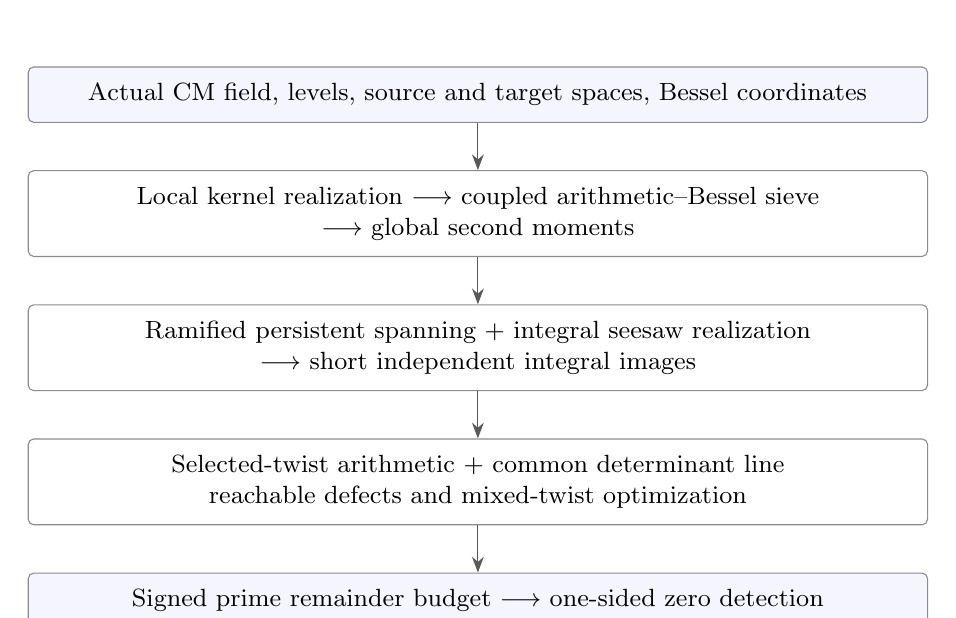
\begin{tikzpicture}[node distance=6mm, every node/.style={font=\small}, box/.style={draw=black!45, rounded corners=2pt, align=center, text width=11cm, inner sep=6pt}, arr/.style={-{Stealth[length=2mm]},black!65}]
\node[box,fill=blue!4] (a) {Actual CM field, levels, source and target spaces, Bessel coordinates};
\node[box,below=of a] (b) {Local kernel realization $\longrightarrow$ coupled arithmetic--Bessel sieve\\ $\longrightarrow$ global second moments};
\node[box,below=of b] (c) {Ramified persistent spanning $+$ integral seesaw realization\\ $\longrightarrow$ short independent integral images};
\node[box,below=of c] (d) {Selected-twist arithmetic $+$ common determinant line\\ reachable defects and mixed-twist optimization};
\node[box,below=of d,fill=blue!4] (e) {Signed prime remainder budget $\longrightarrow$ one-sided zero detection};
\draw[arr](a)--(b);\draw[arr](b)--(c);\draw[arr](c)--(d);\draw[arr](d)--(e);
\end{tikzpicture}
\end{center}
\noindent The arrows denote required implications, not assertions that all their hypotheses have been proved here.

\section{Exact arithmetic scales and Poisson normalization}\label{sec:scales}
Let $E$ be a CM field of degree $2f$, with one chosen complex embedding at every infinite place $v$. Write $|z_v|$ for the ordinary complex modulus, $\N\mathfrak a$ for the absolute ideal norm, and $v_{\mathfrak p}$ for the integer-valued additive valuation at a finite prime. Thus
\begin{equation}\label{eq:norm}
\prod_{v\mid\infty}|z_v|^2=|N_{E/\mathbb Q}(z)|=\prod_{\mathfrak p}(\N\mathfrak p)^{v_{\mathfrak p}(z)}\quad(z\ne0).
\end{equation}
The source defines $n=\rho+1$, rank $k$, $K=k-n^7\geq0$, level $M$, prime $N$, and real archimedean factors $\kappa_v=M\Phi_v(\varpi)/(2\pi i)$, where $\varpi$ generates the different. Set
\begin{equation}
s(v,a)=\frac{|\kappa_v|^{2(\rho-a)}}{N},\quad 0\leq a\leq\rho,\qquad \KK=\prod_v|\kappa_v|.
\end{equation}
Here $\kappa_v$ is not the quadratic Dirichlet character used at the analytic endpoint. By the norm of the different and $\mathrm{rd}(E)=|\mathrm{disc}(E)|^{1/(2f)}$,
\begin{equation}\label{eq:kappa}
\KK=\left(\frac{M\,\mathrm{rd}(E)}{2\pi}\right)^f.
\end{equation}
This is the source's \texttt{prod\_\allowbreak abs\_\allowbreak realM} in \texttt{GlobalSieve.lean} \cite{globalsieve}. The admissible setting has $1\leq|\kappa_v|\leq b^{23}$ and $N\leq b^{60n}$, where $b$ is its size parameter. Define $c_{j,v}=\prod_{a<j}s(v,a)$ and $C_j=\prod_v c_{j,v}$. Direct calculation gives
\begin{align}
\prod_v s(v,a)&=\KK^{2(\rho-a)}N^{-f},\\
\frac{\prod_v s(v,a+1)}{\prod_v s(v,a)}&=\KK^{-2}\quad(a<\rho),\\
C_j&=\KK^{j(2\rho-j+1)}N^{-fj},\quad 0\leq j\leq n.\label{eq:prefix}
\end{align}
Write $c_E=\vol(\widehat{\OO}_E)>0$ in the source's Haar normalization. Its one-entry Poisson factor is $P_a=c_E/\prod_v s(v,a)^2$, so
\begin{equation}\label{eq:poissprod}
\Pi_i:=\prod_{a<i}P_a=c_E^i N^{2fi}\KK^{-2i(2\rho-i+1)},\qquad \Pi_0=1.
\end{equation}
\status{(S) for the scale and Haar conventions; (P) for the consequences above. No averaging or independence between embeddings is required.}

\section{Norm exclusion and anisotropic ideal packing}\label{sec:packing}
For $z\in E^\times$, let $\mathfrak d(z)=\prod_{\mathfrak p}\mathfrak p^{\max(0,-v_{\mathfrak p}(z))}$ denote the denominator ideal. Equation \eqref{eq:norm} gives
\begin{equation}\label{eq:denom}
\prod_v|z_v|^2\geq(\N\mathfrak d(z))^{-1}.
\end{equation}
For an integral ideal $\mathfrak d\ne0$ and radii $R_v>0$, let
\[
\mathcal B(R)=\{z\in\mathbb C^f:|z_v|\leq R_v\ (\forall v)\},\qquad V=\N\mathfrak d\prod_v R_v^2.
\]
This $V$ is a dimensionless product of scales, not the actual Haar volume of a fundamental domain; discriminant factors in the latter should not be conflated with $V$.
\begin{theorem}[Anisotropic ideal packing]\label{thm:packing}
For $0\leq\eta$ and $V$ as above,
\begin{equation}\label{eq:pack}
\#\bigl(\mathfrak d^{-1}\cap\mathcal B(R)\setminus\{0\}\bigr)
\leq 9^f V\,\mathbf1_{V\geq1}\leq9^f V^{1+\eta}.
\end{equation}
\end{theorem}
\begin{proof}
If $z\in\mathfrak d^{-1}\setminus\{0\}$, then $z\mathfrak d$ is a nonzero integral ideal; hence $|N(z)|\N\mathfrak d\geq1$. Thus no nonzero point lies in $\mathcal B(R)$ if $V<1$. For distinct points $z,w$ of $\mathfrak d^{-1}$ the same argument applies to $z-w$. After coordinate-wise rescaling by $R_v^{-1}$ their separation in the maximum of the complex moduli is at least $\delta=V^{-1/(2f)}$. Closed balls of radius $\delta/2$ about these points have disjoint interiors and fit into the ball of radius $1+\delta/2$ about zero. Their volumes scale as the $2f$-th power of the radius. For $V\geq1$, the resulting count is at most $(1+2/\delta)^{2f}\leq 3^{2f}V$. Finally $V\leq V^{1+\eta}$ on $V\geq1$.
\end{proof}
\begin{corollary}[Adelic frequency exclusion]
For a nonzero frequency $\nu$ and positive scales $s(v,a)$,
\begin{align}
\prod_v\frac{|\nu_v|}{s(v,a)}&\geq\frac{N^f}{\KK^{2(\rho-a)}\sqrt{\N\mathfrak d(\nu)}},\\
\sum_v\left(\frac{|\nu_v|}{s(v,a)}\right)^2&\geq f\left(\frac{N^f}{\KK^{2(\rho-a)}\sqrt{\N\mathfrak d(\nu)}}\right)^{2/f}.
\end{align}
\end{corollary}
\begin{proof}Divide \eqref{eq:denom} by the squared scale product and use the arithmetic--geometric mean inequality.\end{proof}
This is a precise sense in which finite-place arithmetic can rule out simultaneous near-zero archimedean frequencies. It does not prohibit a tiny frequency at one embedding if other embeddings or the denominator compensate. The sequence $\nu=1/L$ over $\mathbb Q$ (or any fixed CM field) demonstrates the necessity of the denominator term.

The theorem is a coarse count, not an asymptotic lattice discrepancy result. Admissible lattices and multiplicative separation are classical (Skriganov, Widmer); see \cite{skriganov,widmerweak,widmercount,barroero}. Our intended contribution is the exact application to the coupled Bessel decay with its finite denominator factor, not priority for the packing principle.

\section{The coupled arithmetic--Bessel frequency estimate}\label{sec:kernel}
Let $T$ be the finite set of finite places and $\OO_{E,T}$ the ring of $T$-integers. For $\nu\in\OO_{E,T}\setminus\{0\}$ put
\[
J_T(\nu)=\prod_{\mathfrak p\in T}(\N\mathfrak p)^{v_{\mathfrak p}(\nu)},\quad I_{\rm out}(\nu)=\prod_{\mathfrak p\notin T}(\N\mathfrak p)^{v_{\mathfrak p}(\nu)}\in\mathbb Z_{\geq1}.
\]
With the usual semilocal ideal-index convention, $J_T$ is the generalized index $[\OO_T:\nu\OO_T]$, where here $\OO_T=\prod_{\mathfrak p\in T}\OO_{E_{\mathfrak p}}$. The denominator index $[\OO_T:\OO_T\cap\nu^{-1}\OO_T]$ equals $\N\mathfrak d(\nu)$ (the source only needs the corresponding inequality). The exact cancellation is
\begin{equation}\label{eq:cancel}
\frac{J_T(\nu)^{K/2}}{\prod_v|\nu_v|^K}=I_{\rm out}(\nu)^{-K/2}.
\end{equation}
This is the signed norm bookkeeping behind the source's \texttt{frequencyDecay}, \texttt{frequency\_\allowbreak term\_\allowbreak le} and \texttt{boundsDecay\_\allowbreak prod}. The exponent $K$ appears on both sides; it is not necessary to bound the two sides separately.

\subsection{The exact majorant interface}
For coordinate $a$ and nonzero complex frequency scaling coefficients $c_v$, put $q_v=s(v,a)/|c_v|$ and $Q=\prod_v q_v$. The frequency is read at infinity as $\xi_v=c_v\nu_v/s(v,a)$, and at $T$ as $\nu$. In the source's \texttt{GlobalSieve.lean}, the product decay is the archimedean factor
\[\prod_v \mathrm{scaledVolumeRatio}\,b^{2000 n^9} \mathrm{dampedPower}_K(|\xi_v|^{-1})\]
times the finite factor $b^{n^9f} J_T(\nu)^{K/2}/\mathrm{denomIndex}^3$, where $\mathrm{dampedPower}_K(z)=z^K\min(1,z^6)$. Hence the following majorant is valid for that product decay:
\begin{equation}\label{eq:beta}
\beta_a(\nu;c)\leq A Q^K\frac{I_{\rm out}(\nu)^{-K/2}}{(\N\mathfrak d(\nu))^3}\prod_v\min\left(1,\frac{q_v^6}{|\nu_v|^6}\right),\qquad A=\mathrm{scaledVolumeRatio}^f b^{2001n^9f}.
\end{equation}
If the local estimates have larger explicit normalization factors, they must be retained in $A$. This is a majorant, not an identity for the signed oscillatory kernel itself. The local Fourier decay and orbital-density axioms are substantive source inputs; deriving the estimate below does not prove them.

\begin{theorem}[Packing-integrated Bessel majorant]\label{thm:bessel}
Suppose \eqref{eq:beta} holds, $K\geq0$ and $0\leq\eta<1$. Then
\begin{equation}\label{eq:bessel}
\sum_{\nu\in\OO_{E,T}\setminus\{0\}}\beta_a(\nu;c)\leq A C_\eta^f Q^{K+2+2\eta},\qquad C_\eta=\frac{54}{4-2\eta}\zeta(2-\eta)^2.
\end{equation}
In particular, for $\eta=0$ the constant can be replaced by $37^f$.
\end{theorem}
\begin{proof}
The elementary layer-cake identity is $\min(1,r^{-6})=\int_1^\infty 6u^{-7}\mathbf1_{r\leq u}\,du$ for $r>0$. Fix an integral ideal $\mathfrak d$. By Tonelli and Theorem \ref{thm:packing} applied to $R_v=q_vu_v$,
\begin{align*}
\sum_{\mathfrak d(\nu)=\mathfrak d}\prod_v\min(1,(q_v/|\nu_v|)^6)
&\leq9^f(\N\mathfrak d)^{1+\eta}Q^{2+2\eta}
\prod_v\int_1^\infty6u^{-5+2\eta}\,du\\
&=\left(\frac{54}{4-2\eta}\right)^f(\N\mathfrak d)^{1+\eta}Q^{2+2\eta}.
\end{align*}
The sum is over nonzero elements; $\mathfrak d(\nu)=\mathfrak d$ implies membership in $\mathfrak d^{-1}$. Discard $I_{\rm out}^{-K/2}\leq1$ and sum with the weight $(\N\mathfrak d)^{-3}$. Enlarging the denominator ideals to all nonzero integral ideals gives $\zeta_E(2-\eta)$, which is finite for $\eta<1$. At every rational prime, the Euler factors are bounded by those of $\zeta(s)^{2f}$ for $s>1$, since the number of prime ideals over a rational prime is at most $2f$ and their residue degrees are at least one. This proves \eqref{eq:bessel}. Finally $(27/2)\zeta(2)^2<37$.
\end{proof}
\status{(P) as a standalone summation theorem; (S/C) when used for the actual orbital-density kernels. The estimate remains valid for $Q>1$, but extra powers only improve attenuation if $Q<1$ or if comparing decreasing relative depth scales. The endpoint $\eta=1$ is not justified: the ideal sum reaches its pole.}

\subsection{The exceptional S-unit graph: a valid but optional refinement}
For $t,s\in\OO_{E,T}^\times$, $t\ne s$, and $M$ a $T$-unit (as follows from the integral rational integer $M$ and $M^{-1}\in\OO_{E,T}$), set $\nu=(t^{-1}-s^{-1})/M$. Outside $T$,
\begin{equation}v_{\mathfrak p}(\nu)=v_{\mathfrak p}(s-t).\end{equation}
The pairs with $I_{\rm out}(\nu)=1$ satisfy $u+v=1$ with $u=t/s$ and $v=(s-t)/s$ both $T$-units. The Beukers--Schlickewei bound \cite{beukers} for a subgroup of $(\mathbb C^\times)^2$ of rank $r$ gives at most $2^{8(r+1)}$ solutions. Dirichlet's unit theorem gives rank $r_T=f-1+|T|$ for $\OO_{E,T}^\times$, so the exceptional graph has degree at most $\Delta_T=2^{8(2r_T+1)}$ for any fixed $s$. Outside this graph the factor in \eqref{eq:cancel} is at most $2^{-K/2}$.

For comparison with the older height-majorization method define
\[H(\nu)=\N\mathfrak d(\nu)\prod_v\max(1,|\nu_v|)^2.\] The residual in \eqref{eq:beta} is at most $\prod_v\max(1,q_v)^6 H(\nu)^{-3}$ after including the denominator term. Thus with $C'_a=A Q^K\prod_v\max(1,q_v)^6$ and $L_T=\sum_{\nu\ne0,\nu\in\OO_{E,T}}H(\nu)^{-3}$,
\begin{equation}\label{eq:sunit}
\mathcal O_a\leq C'_a[\min(\Delta_T,L_T)+2^{-K/2}L_T]\sum_tW_t^2
\end{equation}
for the weighted off-diagonal sum defined in the next section. Indeed $2W_tW_s\leq W_t^2+W_s^2$ bounds the exceptional graph by its degree; convolution supplies the $L_T$ alternative and the damped complement. The same packing-layer method with $q_v=1$ bounds $L_T\leq37^f$. This graph is not a classification of every global near return: it concerns the reciprocal frequencies of the main-term sieve. Enlarging $T$ changes the graph; the S-unit bound may be worse than the height bound. Theorem \ref{thm:bessel} bypasses this classification entirely.

\section{Weighted reciprocal convolution and the head hierarchy}\label{sec:recurrence}
\begin{proposition}[Weighted inverse-coordinate convolution]\label{prop:conv}
Let $A_0\subset E^\times$ be finite, let $W_t\geq0$ for $t\in A_0$, and let $F$ be a nonnegative summable function on the additive group $E$, with $F(0)=0$. Then
\begin{equation}\label{eq:conv}
\sum_{s\ne t} W_sW_t F((t^{-1}-s^{-1})/M)\leq \|F\|_1\sum_tW_t^2.
\end{equation}
\end{proposition}
\begin{proof}Place $w(t^{-1}/M)=W_t$ and extend by zero; the map is injective. Group the ordered pairs by frequency. The result is $\sum_\nu F(\nu)\sum_z w(z)w(z-\nu)$. For each $\nu$, Cauchy--Schwarz bounds the inner sum by $\|w\|_2^2$.\end{proof}
If $\sum W_t^2>0$, the saving against $\|F\|_1(\sum W_t)^2$ is the factor $N_{\rm eff}=(\sum W_t)^2/\sum W_t^2$. No uniform lower bound greater than one is automatic. For the source's \texttt{re\_\allowbreak le\_\allowbreak of\_\allowbreak last\_\allowbreak entries\_\allowbreak ne}, the actual bound before replacing the frequency by its sum is precisely $\beta_a(\nu;M)$ times the two head weights; hence grouping the latter by terminal coordinate is valid at this interface.

\subsection{Exact depth factors}
The admissible Poisson frequency scales satisfy $|c_v|^{-1}\leq |\kappa_v|/M$, whereas the different-terminal-entry term uses $c_v=M$. Define upper products
\begin{align}
Q_a^P&=\frac{\KK^{2(\rho-a)+1}}{(MN)^f}=Q_0^P\KK^{-2a},\\
Q_a^O&=\frac{\KK^{2(\rho-a)}}{(MN)^f}=Q_0^P\KK^{-(2a+1)}.
\end{align}
The majorant is monotone in every $q_v$ for $K\geq0$. Let $L=K+2+2\eta$, $q=\KK^{-L}$, and $\epsilon_0=A C_\eta^f(Q_0^P)^L$. Theorem \ref{thm:bessel} gives
\begin{equation}\label{eq:depth}
\epsilon_a^P\leq\epsilon_0q^{2a},\qquad \epsilon_a^O\leq\epsilon_0q^{2a+1}.
\end{equation}
Without the packing improvement, the source's height estimate gives the same depth structure with $L=K$ and $\epsilon_0=\mathrm{decayConst}\,b^{2002n^9f}$, where $\mathrm{decayConst}=\mathrm{scaledVolumeRatio}^f(Q_0^P)^K$. We use the same local kernel axioms throughout. No local normalization is changed.

\subsection{Arithmetic head products via the same packing principle}
Let $p=(t_0,\ldots,t_{i-1})$ be a head of length $i\leq\rho$, and $\delta_j=\prod_{a<j}t_a$ for $1\leq j\leq i$. Let $B=b^{60n^2}$ and $m_0=n^6$ (this exponent is not the number of lifts). The source's \texttt{globalWeight} vanishes unless $\delta_j$ is integral at $T$ and $|c_{j,v}\delta_{j,v}|\leq B$ at every $v$, for each prefix $j$. Since the entries are integral off $T$, the nonzero-weight prefixes are nonzero global algebraic integers. The prefix map is injective, with $t_{j-1}=\delta_j/\delta_{j-1}$ and $\delta_0=1$.

By Theorem \ref{thm:packing} with $\mathfrak d=\OO_E$, the number of possible nonzero prefixes at depth $j$ is bounded by
\begin{equation}\label{eq:headcount}
9^f B^{2f}C_j^{-2}\mathbf1_{B^{2f}C_j^{-2}\geq1}.
\end{equation}
For each prefix, the finite and archimedean weight factors multiply to at most
\begin{align*}
&\left[J_T(\delta_j)^{1/2}\prod_v\max(1,|c_{j,v}\delta_{j,v}|^{-1})\right]^{m_0}\\
&\quad\leq \left[\prod_v\max(|\delta_{j,v}|,c_{j,v}^{-1})\right]^{m_0}\leq B^{m_0f}C_j^{-m_0},
\end{align*}
using $J_T^{1/2}\leq\prod_v|\delta_{j,v}|$ and $B\geq1$. Thus
\begin{equation}\label{eq:headsum}
S_i:=\sum_p\Lambda_i(p)\leq\prod_{j=1}^i9^f B^{(m_0+2)f}C_j^{-(m_0+2)}.
\end{equation}
If any indicator in \eqref{eq:headcount} vanishes, $S_i=0$. The empty head has weight one. This bound enlarges the prefix domain to the product of all feasible prefix sets; it does not assert independence. Substituting \eqref{eq:prefix} gives the fully explicit exponent
\begin{align}
\log S_i\leq &\,if\log9+i(m_0+2)f\log B\\
&-(m_0+2)\left[\frac{i(i+1)(3\rho+1-i)}3\log\KK-\frac{fi(i+1)}2\log N\right].\label{eq:headlog}
\end{align}
The sum of $j(2\rho-j+1)$ was evaluated exactly. Since $|\kappa_v|\geq1$ and $N\leq b^{60n}$, $c_{j,v}^{-1}\leq B$ for $j\leq\rho$. Equation \eqref{eq:headsum} is therefore no worse than $9^{fi}B^{2(m_0+2)fi}$; one may always take its minimum with the source's bound $b^{130n^9f}$. The exact head-volume expression may improve the bound in parts of parameter space, but no uniform final exponent gain is asserted.

\subsection{First-coordinate dominance of the global sieve}
Write $J_i$ for the source's global head kernels and $D_i$ for \texttt{densitySum}: $D_0$ is the real bottom mass; for $i>0$, $D_i$ sums over pairs of heads of length $i$ whose last entry is common. Let $\Lambda_i$ be the nonnegative weights of the actual global sieve system. The one-sided Poisson step and the off-diagonal decomposition in \texttt{densitySum\_\allowbreak succ\_\allowbreak le} and \texttt{re\_\allowbreak sum\_\allowbreak sum\_\allowbreak le\_\allowbreak densitySum\_\allowbreak add} imply
\begin{equation}\label{eq:recurrence}
D_{i+1}\leq P_i\left[D_i+\epsilon_i^P S_i^2+\mathbf1_{i\geq1}\epsilon_{i-1}^O\sum_t W_{i,t}^2\right],
\end{equation}
where $W_{i,t}=\sum_{p:\,p_{i-1}=t}\Lambda_i(p)$ and $0\leq i<n$. The indexing is crucial: the preceding terminal coordinate is at depth $i-1$, not $i$. The Poisson term uses the full pair-weight bound; convolution applies specifically to the reciprocal off-diagonal term. In the empty-head case the off-diagonal sum is empty and $S_0=1$.

The source supplies $S_i^2\leq \Gamma\Pi_i$ for $i\leq\rho$, with $\Gamma=b^{400n^9f}$ (\texttt{sq\_\allowbreak sum\_\allowbreak globalWeight\_\allowbreak le}). More generally one may use $\Gamma_i=S_i^2/\Pi_i$ and $\Gamma_i^{\rm eff}=\sum_t W_{i,t}^2/\Pi_i$. Iterating \eqref{eq:recurrence} gives the refined budget
\begin{equation}\label{eq:exactrec}
\frac{D_n}{\Pi_n}\leq D_0+\epsilon_0+\sum_{i=1}^{n-1}\left(\epsilon_i^P\Gamma_i+\epsilon_{i-1}^O\Gamma_i^{\rm eff}\right).
\end{equation}
For $\KK>1$ and $L>0$, substitute \eqref{eq:depth}, use $\Gamma_i^{\rm eff}\leq\Gamma_i\leq\Gamma$, and sum the finite geometric series, bounding it by the infinite series:
\begin{equation}\label{eq:dom}
D_n\leq\Pi_n\left[D_0+\epsilon_0\left(1+\frac{\Gamma q}{1-q}\right)\right].
\end{equation}
If a uniform mass bound is needed, replace $D_0$ by that bound. When $q=1$, use the finite sum rather than the displayed infinite-series denominator.

In the large-parameter regime of the programme, $\sqrt{x}\leq m\leq2\sqrt{x}$, $x^5\leq r\leq3x^5$, $k=r+1-m$, $n=m/2$ (at admissible integral choices). Thus $k\asymp x^5$, $n^7=O(x^{7/2})$, and $n^9=O(x^{9/2})$. In the subregime $\KK\geq b^{19f}$,
\[
\Gamma q\leq b^{f(400n^9-19L)}=b^{-\Omega(fx^5)}.
\]
In particular the deeper errors collectively contribute an exponentially small multiple of the first-coordinate error. These asymptotics require the displayed lower bound on $\KK$ and the indicated parameter choices; they are not consequences of the packing lemma alone. The same proof works for any deeper-head budget with $\log\Gamma=o(k\log\KK)$.

\subsection{Compatibility with the downstream Siegel normalization}
The source's \texttt{EnergyEstimate.lean} \cite{energy} supplies a normalization with $\mathrm{scaledSiegelConst}$ and the exact product $\Pi_n$. In its original global bound, $\mathrm{decayConst}\,b^{2403n^9f}$ is the sieve contribution. Keeping the original height bound for $\epsilon_0$ and replacing just the recurrence gives $\mathrm{decayConst}\,b^{2002n^9f}(1+o(1))$ in the above asymptotic regime. The source's bound for the scaled Siegel constant times the decay constant absorbs a further $b^{n^9f}$ relative to its identity second moment. Conditional on the unchanged source comparison of that identity moment to the main moment (in particular its $b^{-3kf}$ budget), the resulting normalized contribution is at most $b^{-3kf+2003n^9f}(1+o(1))$. The exponent separation makes it negligible. For the packing bound, its ratio to the bare $\mathrm{decayConst}\,b^{2001n^9f}$ is $C_\eta^f(Q_0^P)^{2+2\eta}$; using $|\kappa_v|\leq b^{23}$, $MN\geq1$, fixed $\eta<1$ and large $n$, this is bounded by $b^{n^9f}$. Thus the same first-coordinate budget remains available in that regime even if $Q_0^P>1$. No independent proof of Siegel's step or of the non-main-cell estimates is claimed.
\status{(P) convolution, prefix bounds and recurrence algebra; (S) the actual local sieve identities, scale axioms, original head allowance and normalization; (C) the proposed replacement in the global second-moment proof.}
\section{Coherence, interference and centered second moments}\label{sec:coherence}
The previous sections retain the actual finite-place and archimedean factors in a nonnegative majorant. They do not use cancellation of signed amplitudes beyond the local Fourier estimates. This section records the more ambitious routes considered and the exact hypotheses they require.

\subsection{Coherent Fourier representation}
Suppose a kernel on reciprocal coordinates $z_t=t^{-1}/M$ has the form $F(z_t-z_s)$ where $F(z)=\int e^{2\pi i\langle z,\xi\rangle}\,d\mu(\xi)$ for a finite positive measure $\mu$. Then
\begin{equation}\label{eq:coherent}
\sum_{t,s}c_t\overline{c_s}F(z_t-z_s)=\int\left|\sum_t c_t e^{2\pi i\langle z_t,\xi\rangle}\right|^2d\mu(\xi).
\end{equation}
This follows by expanding the square and interchanging finite sums with the integral. It preserves correlations exactly. For the actual coupled Bessel kernel the factors depend on both heads, not merely the reciprocal difference. Translation invariance and positive definiteness of a single scalar function cannot be assumed; even an operator-valued realization requires proof. The absolute majorant in Section \ref{sec:kernel} is not evidence for the positivity of its signed counterpart.

\subsection{Tensor Gram realization}
\begin{proposition}
If $K_1(p,q)=\langle u_p,u_q\rangle$ and $K_2(p,q)=\langle v_p,v_q\rangle$ are Gram kernels, their pointwise product is a Gram kernel for $u_p\otimes v_p$. In the convention that the inner product is linear in its first argument,
\begin{equation}\label{eq:tensor}
\sum_{p,q}c_p\overline{c_q}K_1(p,q)K_2(p,q)=\left\|\sum_p c_p u_p\otimes v_p\right\|^2.
\end{equation}
For nonzero features their normalized absolute pairwise coherence is exactly the product of the individual coherences.
\end{proposition}
\begin{proof}The Hilbert tensor product inner product factors. Expansion of the squared norm proves the identity; normalizing the factors proves the coherence statement.\end{proof}
This is the Schur product theorem in a feature-space representation. The source's \texttt{EnergyEstimate.lean} uses positive orbital-density forms on heads with common terminal entry. Where those forms really are Gram kernels, this realization is available. Extending it to all near returns and non-main branches requires a separate proof. Two all-ones Gram matrices give an all-ones product of rank one: positivity itself supplies no independent directions. The promising target is complementary separation: a configuration poorly distinguished geometrically should be distinguished at finite places, or vice versa, with a summable coherence bound after the true arithmetic weights are inserted. For example, if a normalized Gram matrix has row sums of absolute off-diagonal entries at most $\varepsilon<1$, then its eigenvalues lie in $[1-\varepsilon,1+\varepsilon]$ by the elementary row-sum bound on the operator norm. Establishing such a bound is the hard arithmetic step, not the Gram identity.

\subsection{Conditional coherence and exact character cancellation}
Let $G$ be a finite abelian group and $r(t)\in G$ a label. For vectors $a_t$ in a Hilbert space, orthogonality of characters gives
\begin{equation}\label{eq:char}
\frac1{|G|}\sum_{\chi\in\widehat G}\left\|\sum_t\chi(r(t))a_t\right\|^2
=\sum_{g\in G}\left\|\sum_{r(t)=g}a_t\right\|^2.
\end{equation}
Thus all interactions between distinct labels vanish exactly. More generally, compact group representations split into isotypic components; an intertwiner between inequivalent irreducibles vanishes by Schur's lemma. Brox's frontier notes \cite{broxfrontier} report such a concrete distinct-type cancellation in the original zero-Gram branch. This is source-derived progress for that branch; it is not a claim of orthogonality for the rewritten nonzero-Gram branches.

A plausible decomposition uses classes of heads sharing first-coordinate and congruence invariants. Let $A_h(\xi)=\sum_{t\in h}w_t e^{2\pi i\langle z_t,\xi\rangle}$. Then the global energy in \eqref{eq:coherent} is the sum of the within-class energies and cross terms $\sum_{h\ne h'}\langle A_h,A_{h'}\rangle_{L^2(\mu)}$. Far returns might be treated by Bessel attenuation and near returns by exact compact-type orthogonality. The label must come from a genuine action or quotient of the actual arithmetic system with compatible weights and maps. There are two obstructions to an arbitrary modulation. First, the standard adelic additive character is trivial on the diagonal copy of $E$; globally rational frequencies cannot be killed merely by pretending that a local additive phase remains nontrivial globally. Second, the averaging idempotent carries a factor $1/|G|$, potentially producing denominators at coefficient primes dividing $|G|$. Rational orthogonality does not imply integral orthogonality.

\subsection{Centered Gram energy}
For a positive semidefinite Gram operator $G$ on a $D$-dimensional target with $\Tr G>0$, set $A=D G/\Tr G$. Then
\begin{equation}\label{eq:center}
\|A-\Id\|_{\rm HS}^2=\frac{D^2\Tr(G^2)}{(\Tr G)^2}-D.
\end{equation}
This follows from $\Tr A=D$. In particular if $\Tr(G^2)\leq(1+\varepsilon)(\Tr G)^2/D$, the number of eigenvalues with $|\lambda(A)-1|\geq\tau>0$ is at most $\varepsilon D/\tau^2$. Hence a large spectrally well-conditioned subspace is obtained even if the worst direction is not controlled. Also Cauchy--Schwarz gives $\rk G\geq(\Tr G)^2/\Tr(G^2)$. The promising direct target is the excess energy $\Tr(G^2)-(\Tr G)^2/D$, rather than separate crude bounds on two enormous quantities. Any direct cancellation must use the same operator, normalization, probability weights and local masses in both terms. Otherwise the difference contains a false residual.

\subsection{Schur-complement obstruction}
For a block positive matrix $G=\begin{pmatrix}A&B\\B^*&D_0\end{pmatrix}$ with $D_0$ invertible,
\begin{equation}\det G=\det D_0\det(A-BD_0^{-1}B^*).\end{equation}
This is the algebraic analogue of eliminating internal variables of a passive network. However $G_\varepsilon=\begin{pmatrix}1&\sqrt\varepsilon\\\sqrt\varepsilon&\varepsilon\end{pmatrix}$ is positive semidefinite, its off-diagonal tends to zero, and its effective first block is identically zero. Small absolute coupling is insufficient; the relevant relative quantity is $\|A^{-1/2}BD_0^{-1/2}\|$ on the nondegenerate supports. In the singular case the Moore--Penrose inverse and range conditions are needed. We therefore do not use Schur elimination as a replacement for actual global moment estimates.
\status{(P) the identities, bounds and counterexamples in this section; (C/O) the coherent and complementary-separation applications beyond the source's verified common-terminal and distinct-type cases.}

\section{Direct ramified-source persistent spanning}\label{sec:spanning}
Let $S$ be the source space, $S_{\rm ram}\subset S$ the integral-relevant ramified source subspace, and $T_0$ the target (not the finite-place set $T$). The actual translate maps are $A_t:S\to T_0$, indexed by the probability measure on translates from the common Poincar\'e construction. Write $D=\dim T_0$ and $B_t=A_t|_{S_{\rm ram}}$. The proposed procedure restricts the source before selection, so the selected short images already have the source restriction required by the seesaw. The source's \texttt{ShortAndEnough.lean} supplies a retained-dimension estimate of the form $(1-4/b^2)D$ using a codimension allowance for the ramified restriction. The programme seeks to recover that performance directly, without charging the full ramification codimension independently after each translate. The earlier source reading gives a codimension fraction bounded by $f/(N-1)$, and $\alpha\leq b^{-8}$ in the intended large-parameter regime; the precise parameter inference must be checked when importing the lemma.

\subsection{Compression and the lost first moment}
Let $P_{\rm ram}$ project orthogonally onto $S_{\rm ram}$ and set $G_{\rm full}=\mathbb E_t A_tA_t^*$ and $G_{\rm ram}=\mathbb E_t A_tP_{\rm ram}A_t^*$. Then
\begin{equation}\label{eq:compress}
0\preceq G_{\rm ram}\preceq G_{\rm full},\qquad \Tr G_{\rm ram}^2\leq\Tr G_{\rm full}^2.
\end{equation}
The trace-square inequality follows from $\Tr(Y^2-X^2)=\Tr((Y-X)(Y+X))\geq0$ for $0\preceq X\preceq Y$. The exact trace loss is
\begin{equation}\label{eq:traceloss}
\Tr(G_{\rm full}-G_{\rm ram})=\mathbb E_t\|A_t(\Id-P_{\rm ram})\|_{\rm HS}^2.
\end{equation}
It is not bounded by the dimension fraction $\alpha=1-\dim S_{\rm ram}/\dim S$ times the full trace without further information. For example, a rank-one map supported only on the removed direction loses all its trace even for arbitrarily small $\alpha$. If a source symmetry gives $\mathbb E A_t^*A_t=\lambda\Id_S$, then the loss is exactly $\alpha\Tr G_{\rm full}$, and the relative second moment normalized by squared trace increases by at most $(1-\alpha)^{-2}$. A weaker approximate symmetry can suffice if its loss is explicitly budgeted. This distinction is necessary for a valid direct-ramified argument.

\subsection{Saturated information and persistent selection}
For any scale $\lambda>0$, put
\begin{equation}\label{eq:saturation}
C_t=\min(\lambda^{-1}B_tB_t^*,\Id),
\end{equation}
where the minimum is defined by spectral functional calculus. Then $0\preceq C_t\preceq\Id$ and $\operatorname{ran}C_t=\operatorname{ran}B_t$. For every orthogonal projector $Q$ onto the current unobserved subspace,
\begin{equation}\label{eq:rankinfo}
\rk(QB_t)\geq\Tr(QC_tQ).
\end{equation}
Indeed $QC_tQ$ is a positive contraction, with rank equal to the rank of $QB_t$ because $C_t$ and $B_tB_t^*$ have the same support. Each eigenvalue is at most one. Choosing a translate with at least the average trace guarantees a decrease in unobserved dimension of at least that trace. More explicitly, let $C=\mathbb E C_t$. If $C\succeq c\Id$ then for an unobserved dimension $r_j$ at step $j$ there is a translate with $r_{j+1}\leq(1-c)r_j$, giving $r_j\leq D(1-c)^j$. If only $\Tr((c\Id-C)_+)\leq\delta$, then $\Tr(QCQ)\geq cr_j-\delta$, so the same procedure gives $r_j\leq (1-c)^jD+\delta/c$ for $0<c\leq1$. This proves a genuine persistent-measurement lemma on the changing residual subspace.

There is a scale obstruction: $\Tr C_t\leq\dim S_{\rm ram}$, so $c$ cannot exceed the average rank fraction $\dim S_{\rm ram}/D$. A low-rank source cannot be made nearly isometric on the entire target by artificial normalization of the saturated contraction. Nor does a scalar bound on $\Tr(\mathbb E B_tB_t^*)^2$ alone yield a uniform lower bound on $\mathbb E C_t$. For instance, let $B_tB_t^*=M\Id$ with probability $1/M$ and zero otherwise: its average is $\Id$, but for $\lambda=1$ the averaged saturation is $\Id/M$. In applications one needs the actual translate-wise deficit/shortness bound or a moment of individual maps, not merely the second moment of the average.

One useful sufficient condition follows from the scalar inequality $\min(x,1)\geq x-x^2/4$ for $x\geq0$. Functional calculus gives
\[
C\succeq\lambda^{-1}G_{\rm ram}-(4\lambda^2)^{-1}\mathbb E(B_tB_t^*)^2.
\]
This supplies an explicit target for the actual second moments, if the individual-map second moment is available in the required normalization. It is not automatically the same as the Bessel moment in Section \ref{sec:recurrence}. The intended gain of the persistent framework is to recover independent directions without inflating the rank by energetic outliers, while restricting to the actual integral source. It cannot manufacture the missing arithmetic covariance.
\subsection{A direct ramified deficit transfer and explicit greedy recurrence}
The source-deficit formulation in Brox's revised plan \cite{broxplan} gives a stronger way to avoid the unjustified first-moment symmetry assumption in \eqref{eq:traceloss}. Let $d_S=\dim S$, $d_R=\dim S_{\rm ram}=(1-\alpha)d_S>0$. Assume the actual full-source maps satisfy the mean positive source-deficit and covariance hypotheses
\begin{align}
\mathbb E_t\Tr(\Id_S-A_t^*A_t)_+&\leq\delta_S d_S,\\
\Tr G_{\rm full}^2&\leq(1+\epsilon)d_S^2/D.
\end{align}
Here $X_+$ is the positive part of a self-adjoint operator. These are distinct hypotheses: the first is not simply a covariance trace bound. For any self-adjoint $H$, the trace of its positive part equals $\max_{0\preceq Q\preceq I}\Tr(QH)$. Compressing to a subspace restricts the set of admissible $Q$ in this variational expression, so
\begin{equation}
\Tr(\Id_{S_{\rm ram}}-B_t^*B_t)_+\leq\Tr(\Id_S-A_t^*A_t)_+.
\end{equation}
Together with \eqref{eq:compress}, this transfers both hypotheses directly to the ramified source with
\begin{equation}
\delta_R=\frac{\delta_S}{1-\alpha},\qquad 1+\epsilon_R=\frac{1+\epsilon}{(1-\alpha)^2}.
\end{equation}
Use $\lambda=1$ in \eqref{eq:saturation} (the same near-isometry normalization as the deficit hypothesis). The nonzero spectra of $B_t^*B_t$ and $B_tB_t^*$ agree, so
\begin{align}
\Tr C&=d_R-\mathbb E_t\Tr(\Id_{S_{\rm ram}}-B_t^*B_t)_+\geq(1-\delta_R)d_R,\\
\Tr C^2&\leq\Tr G_{\rm ram}^2\leq(1+\epsilon_R)d_R^2/D.
\end{align}
It follows by expanding the square that
\begin{equation}
\left\|C-\frac{d_R}{D}\Id\right\|_{\rm HS}^2
\leq(2\delta_R+\epsilon_R)\frac{d_R^2}{D}.
\end{equation}
For an unobserved projector $Q$ of rank $r$, Hilbert--Schmidt Cauchy--Schwarz now gives
\begin{equation}\label{eq:directram}
\Tr(QC)\geq\frac{d_R}{D}r-d_R\sqrt{(2\delta_R+\epsilon_R)r/D}.
\end{equation}
Choose $\eta_R\in(2\delta_R+\epsilon_R,1)$ and write $c_R=(d_R/D)(1-\sqrt{(2\delta_R+\epsilon_R)/\eta_R})$. While $r\geq\eta_RD$, the right side of \eqref{eq:directram} is at least $c_Rr$. Equation \eqref{eq:rankinfo} therefore supplies a greedy selection reducing $r$ to at most $(1-c_R)r$ at each step before the threshold. In the case $0<c_R<1$, at most $\lceil\log(1/\eta_R)/[-\log(1-c_R)]\rceil$ such steps suffice; $c_R=1$ gives complete recovery in one step. This uses a positive source deficit, not a conjectured proportional trace loss. It is a direct quantitative transfer to the restricted source. The actual arithmetic moments, translate-wise shortness and the exact number-of-translates budget must still match the source's choices. The bound is a proved abstract supplier, not evidence that those arithmetic hypotheses hold. The underlying covering mechanism is closely related to Brox's stated covering lemma, rather than a priority claim for persistent selection.

\status{(P) compression, exact loss, saturation and selection lemmas; (S) the source's original spanning guarantee and restriction interface; (C/O) the desired direct quantitative replacement on the same ramified arithmetic maps.}

\section{Integral theta realization and clearing indices}\label{sec:theta}
The determinant route requires a common finite-dimensional target $V$ over a coefficient field and a family of theta maps $\Theta_\vartheta:V\to W_\vartheta$ with algebraic structures and Hermitian pairings compatible with coefficient extension. In the earlier source reading the declarations \texttt{New.Data.seesaw\_\allowbreak identity} and \texttt{New.Data.exists\_\allowbreak err\_\allowbreak gaugeLe\_\allowbreak compositeLift} in the readable development supply the seesaw and valuation estimates. We record the full needed interfaces rather than assume that any ordinary theta map satisfies them.

\subsection{Common-scalar seesaw and simultaneous integrality}
The required seesaw compares the Poincar\'e map $\mathcal P$ with the integral composite theta construction, on every ramified source vector $\phi$:
\begin{equation}\label{eq:seesaw}
\Theta_\vartheta\mathcal P\phi=c\,\mathcal T_{\vartheta,\Psi_\vartheta}\phi.
\end{equation}
Here $c\ne0$ is independent of $\vartheta$ and $\phi$; $\Psi_\vartheta$ is finite chain data with the prescribed support, level invariance and integrality outside the permitted conductor. A scalar $c_\vartheta$ varying with the twist is not an innocent replacement: its determinant powers enter the finite-place and archimedean budgets. The arithmetic divisibility supplier gives simultaneous local integral submodules for the allowed twists and chain data, with nonnegative losses $e_p$ whose prescribed total is of the form $\sum_p e_p\log p\leq fa(\log b)^3$ in the source's notation (the parameter $a$ here is a source divisibility parameter, not the coordinate index). The exact coefficient embeddings, conductor exclusions, gauge and index bounds must be carried unchanged when applying the theorem. We do not independently reconstruct its local representation-theoretic proof in this manuscript.

At a coefficient prime $\mathfrak p$, the relevant integrality condition on $V$ is a simultaneous pullback:
\begin{equation}\label{eq:pullback}
L_{\mathfrak p}=\bigcap_{\vartheta\ \mathrm{allowed}}\Theta_\vartheta^{-1}(M_{\vartheta,\mathfrak p}).
\end{equation}
This formula requires the maps to be defined over the appropriate common local coefficient extensions; the lattice property itself needs boundedness and spanning. The source defines integrality using a family of theta lifts rather than postulating a convenient target lattice independent of them. The analytic metric is given by the untwisted theta norm, while the arithmetic lattice must pass all allowed integral tests. This is the concrete compatibility that makes the determinant comparison possible.

\subsection{Exact clearing-index budget}
Let $O$ be a discrete valuation ring with uniformizer $\pi$ and integer-valued valuation $v$. For any lattice $L$ in a finite-dimensional local vector space and finite-index sublattice $L_{\rm int}$, elementary divisors give a basis of $L$ for which $L_{\rm int}$ is generated by $\pi^{e_i}$ times the basis vectors, $e_i\geq0$. Hence
\begin{equation}\label{eq:clear}
\len_O(L/L_{\rm int})=\sum_i e_i=v(\det C),
\end{equation}
where $C$ is a clearing matrix. The exact cost is a sum of elementary divisor exponents, not the rank times the worst exponent. If the valuation is normalized by $v(p)=1$, every module length is divided by the ramification index $v_\pi(p)$; all formulas below then hold with that normalized length. For a pairing matrix $G$, left and right clearing matrices multiply the determinant by their two determinant factors. At conjugate primes the two costs must be accounted for separately; only in the symmetric case are they equal. The source already uses operator-valued clearing determinants. The proposed further economy is to apply \eqref{eq:clear} to the actual lattice generated by the retained short images, rather than a worst-case full-source allowance. This requires the simultaneous integrality and a proof of the colength bound for the selected images.

If $L_1,L_2$ are two integral sublattices of $L$, the injection $L/(L_1\cap L_2)\hookrightarrow L/L_1\oplus L/L_2$ gives a subadditive clearing bound. It is not generally bounded by the maximum of the individual colengths. For example $L_1=\pi^hO\oplus O$ and $L_2=O\oplus\pi^hO$ each have colength $h$, but their intersection has colength $2h$. This distinction matters when collecting multiple twists.
\status{(P) the local index identities; (S) the integral theta interfaces of the pinned construction; (C/O) the common lattice dictionary and reduced arithmetic colength on the actual selected family.}

\section{Adelic volume conservation and reachable congruence defects}\label{sec:reachable}
The source's comparison mechanism involves a good-lift subspace, false lifts and gluing maps. Earlier source readings located the pertinent declarations in \texttt{IntegralTargetForms.lean}, \texttt{TwistedLattice.lean}, \texttt{LongForms.lean}, \texttt{LiftVolumeHeight.lean} and \texttt{NormOfChain.lean}. The following proposition spells out the algebraic identity underlying the reported comparison. The source-specific normalization and Hecke-value ratio are separate arithmetic inputs, not consequences of this proposition.

\begin{proposition}[Exact compression-volume identity]\label{prop:glue}
Let $u:V\to W$ be injective between finite-dimensional Hermitian spaces, let $A=\operatorname{ran}u$ and $P$ be its orthogonal projector. Let $g:H\to W$, $J:V\to H$ satisfy $c g^*u=J$ with $c\ne0$, and put $U=Cgg^*$, $C>0$. Suppose $J$ is injective and write $d=\dim V$, $Z=\det(u^*u)$ in an orthonormal basis of $V$, and $\Delta=\det(PU|_A)$. Then
\begin{equation}\label{eq:glue}
Z\Delta=C^d|c|^{-2d}\det(J^*J).
\end{equation}
\end{proposition}
\begin{proof}
The matrix of $PU|_A$ in the basis formed by the columns of $u$ is $(u^*u)^{-1}u^*Uu$. Its determinant multiplied by $Z$ is $\det(u^*Uu)$. But $u^*Uu=C(g^*u)^*(g^*u)=C|c|^{-2}J^*J$. Take determinants.\end{proof}
For the actual good-lift and gluing maps, write $u_\vartheta,g_\vartheta,J,c_\vartheta,C$. The reported source comparison has a twist-independent factor $C_0$ and a prescribed Hecke-value ratio $\rho_\vartheta$ giving $Z_\vartheta\Delta_\vartheta=C_0\rho_\vartheta^d$ in its normalization. Proposition \ref{prop:glue} verifies the linear-algebra mechanism: obtaining exactly that $C_0$ and $\rho_\vartheta$ depends on the arithmetic gluing, norm and exchange identities. In particular $c_\vartheta$ in this proposition should not be confused with the common scalar in \eqref{eq:seesaw}. The rational splitting, the false-lift exclusion, the algebraicity of the corrected volume and integrality of $U_\vartheta$ are substantive requirements.

\subsection{Measure only the torsion reached by the comparison}
Let $O$ be a DVR, $F$ its fraction field, and let $M_0$ be a full $O$-lattice in $W_F=A_F\oplus B_F$. Think of $M_0$ as the ambient integral lattice after imposing orthogonality to the false lifts, $A_F$ as the good-lift subspace, and $B_F$ as its complement. Assume the decomposition and its projection $P$ are defined over $F$ and put $L=M_0\cap A_F$, $L_B=M_0\cap B_F$. The full projection congruence module is
\begin{equation}\label{eq:cong}
\mathcal C=PM_0/L\simeq M_0/(L+L_B).
\end{equation}
The isomorphism is induced by $P$: it is surjective and $Pm\in L$ precisely when $m\in L+L_B$. These quotients are finite length because the intersection lattices span their respective rational subspaces.

Suppose the actual integral comparison $U$ satisfies $UL\subset M_0$ and $T_U=PU|_{A_F}$ is invertible. Define
\begin{equation}\label{eq:reach}
\mathcal C_U=(L+T_UL)/L\subseteq\mathcal C.
\end{equation}
This is the congruence defect reachable by the operator; it may be strictly smaller than the full congruence module.
\begin{theorem}[Signed local volume defect]\label{thm:signed}
With these hypotheses,
\begin{equation}\label{eq:signed}
-v(\det T_U)=\len_O(\mathcal C_U)-\len_O\bigl(L/(L\cap T_UL)\bigr).
\end{equation}
In particular $-v(\det T_U)\leq\len_O(\mathcal C_U)\leq\len_O(\mathcal C)$.
\end{theorem}
\begin{proof}By the second isomorphism theorem $\mathcal C_U\simeq T_UL/(L\cap T_UL)$. Write $L'=L\cap T_UL$. If $d_L(L')$ denotes the valuation of the determinant of a basis of $L'$ relative to a basis of $L$, then $\len(L/L')=d_L(L')$. Relative to the basis of $T_UL$, the same determinant valuation is $d_L(L')-v(\det T_U)$. Subtract the lengths.\end{proof}
Unlike the usual upper estimate for a denominator, \eqref{eq:signed} retains the favorable numerator term. In a normalized $p$-adic valuation multiply lengths by the reciprocal ramification index, as in Section \ref{sec:theta}. If $U=Cgg^*$ and $cg^*u=J$, then
\begin{equation}\label{eq:reachperiod}
UL=(C/c)gJ(u^{-1}L)
\end{equation}
when the maps, involution and scalar conventions have been transported to the same coefficient field. Therefore it suffices to bound the image of this period lattice modulo $L+L_B$, not necessarily every element of the ambient congruence module. A particularly strong sufficient condition is
\begin{equation}\label{eq:vanish}
(C/c)gJ(u^{-1}L)\subseteq L+L_B.
\end{equation}
Then $\mathcal C_U=0$, so $v(\Delta)\geq0$. This would remove the corresponding projection-denominator loss. It is an explicit arithmetic containment to investigate; it is not yet proved for the actual theta maps.

\subsection{Counterexample to automatic conservation of integrality}
The gluing identity, injectivity, positivity, and even integral bounded comparison operators do not imply \eqref{eq:vanish}. Let $O=\mathbb Z_5$ and choose an integer $a$ with $v_5(1+a^2)=h$ for any prescribed $h\geq1$. Such integers exist by Hensel lifting a root of $a^2+1$ mod $5$ and choosing a lift not solving it modulo $5^{h+1}$. With the ordinary rational dot product let
\[
u=\binom{1}{a},\qquad g=\binom{1}{0},\qquad U=gg^*=\begin{pmatrix}1&0\\0&0\end{pmatrix}.
\]
Then $g^*u=1$, $U$ is integral and positive over $\mathbb R$, and the projection to $A=F u$ is $P=uu^*/(1+a^2)$. Thus $Z=1+a^2$, $\Delta=(1+a^2)^{-1}$ and $Z\Delta=1$ exactly. Yet $-v_5(\Delta)=h$ is unbounded. Here $L=Ou$, $PUL=(1+a^2)^{-1}Ou$, so the reachable module itself has length $h$. No generic refinement by reachable torsion can eliminate the arithmetic bound; an actual additional structure is essential. This also illustrates the difference between positivity at a real place and degeneracy modulo a coefficient prime.
\status{(P) the exact identities, inclusion and counterexample; (S) the existence of the prescribed comparison interface in the source; (O) the uniform bound on the actual reachable defect, including possible cancellation of its signed numerator term.}

\section{Finite Selmer presentations and bounded arithmetic witnesses}\label{sec:selmer}
The selected-twist argument requires control of local projection denominators through congruence/Selmer estimates. We separate the elementary finite-presentation machinery from the deeper arithmetic witnesses. The relevant source supplier was located in the earlier reading under \texttt{New/\allowbreak Congruences/\allowbreak Selmer/\allowbreak OneSystem.lean}, \texttt{Line.lean}, and \texttt{GeneralTheorem.lean}, with the matrix-presentation and sharp-polynomial declarations listed in Appendix \ref{app:source}. The following proposition states the precise conditions under which the elementary reconstruction is valid.

\subsection{A common polynomial cocycle matrix}
\begin{proposition}[Finite polynomial presentation]\label{prop:selmer}
Let $O$ be the ring of integers of a finite extension of $\mathbb Q_\ell$, let $T_0=O^d$, and let $\rho:G_E\to\mathrm{GL}_d(O)$ be continuous and unramified outside a finite set of places $S_0$. Fix a truncation $\ell^L$ and continuous character coordinates $h_j:G_E\to\mathbb Z/\ell^H\mathbb Z$ unramified outside $S_0$. Consider admissible specializations $x_j=\zeta_j-1$ where $\zeta_j^{\ell^H}=1$, possibly over finite coefficient extensions $O'/O$. Suppose that the local conditions and the normalization of cocycles are expressed by polynomial linear equations in their values in the common finite quotient below, and that normalized cocycles represent the desired Selmer classes uniquely. Then the truncated normalized Selmer group is the kernel of a finite matrix $A(x)$ over $O'/\ell^L$, obtained by specializing a matrix with polynomial entries over $O$.
\end{proposition}
\begin{proof}
Replace $G_E$ by its quotient unramified outside $S_0$, enlarging $S_0$ to contain the places over $\ell$ as needed. Take the common open normal subgroup $G_0=\ker(\rho\bmod\ell^L)\cap\bigcap_j\ker h_j$. At every admissible specialization its action on $(O'/\ell^L)^d$ is trivial. On $G_0$, a cocycle is an additive continuous homomorphism into a group killed by $\ell^L$. It kills commutators and $\ell^L$-powers, and hence factors through the maximal abelian exponent-$\ell^L$ quotient of $G_0$. This is finite by the arithmetic finiteness of such quotients for the fixed finite ramification set (class field theory). The kernel is characteristic in $G_0$ and normal in the ambient group. Thus all these cocycles factor through a single finite quotient $G_*$, also after coefficient extension. On this quotient, choose polynomial lifts of the action matrices modulo $\ell^L$, using representatives of $h_j(g)$ in $[0,\ell^H-1]$ and the expression $\rho(g)\prod_j(1+X_j)^{h_j(g)}$. These polynomial expressions need not be a representation before specialization; the group relations hold modulo $\ell^L$ at admissible torsion points, which is all that is needed. Introduce finitely many variables $z(g)$, one vector per element of $G_*$. The cocycle equations are $z(gh)-z(g)-\rho_X(g)z(h)=0$, and the stipulated local linear relations add polynomial rows. Even an infinite list of polynomial rows generates a finitely generated row module since $O[X_1,\ldots,X_s]$ is Noetherian. A finite generating list gives the claimed matrix. The normalization hypothesis identifies its kernel with the Selmer group, rather than merely the larger cocycle space.
\end{proof}
The last hypothesis is not automatic: crystalline or other integral local conditions must actually be identified with these equations. A convenient sufficient normalization for a suitable scalar inertial element uses a unit $\zeta_*^2-1$ in the adjoint or twisted representation context of the source. Actual local representation conditions, including unique normalization and the coefficient extension dictionary, must be verified for the relevant representations. The polynomial-matrix construction cannot replace those conditions by mere residual irreducibility.

\begin{proposition}[Minor-to-length identity]\label{prop:minors}
Let $A(x)$ be an $r\times u$ matrix over $O'$, and $a$ a nonzero element of $O'$. Append $aI_u$ as rows to form $\widetilde A(x)$. Then for $v$ the normalized additive valuation and $\len_v$ the correspondingly normalized module length,
\begin{equation}\label{eq:minors}
\len_v\ker(A(x):(O'/a)^u\to(O'/a)^r)=\min_J v(\det\widetilde A_J(x)),
\end{equation}
where $J$ ranges over all sets of $u$ rows.
\end{proposition}
\begin{proof}Smith normal form for $A(x)$ reduces the kernel to the direct sum of the cyclic kernels of multiplication by its diagonal elementary divisors, with zeros counted as infinite valuation. The length is the sum of the minima of their valuations with $v(a)$. The appended matrix has full column rank; its elementary divisors are the same truncated valuations, so their sum equals the valuation of its ideal of maximal minors.\end{proof}
For a given witness point $x_0$, choose a maximal minor $P(X)$ attaining the minimum at $x_0$. Then $v(P(x_0))=\len_v\operatorname{Sel}_L(x_0)$ and $\len_v\operatorname{Sel}_L(x)\leq v(P(x))$ at every admissible point. This is the exact sharp polynomial interface. If the full divisible-coefficient Selmer module $H$ is a torsion module over a DVR and $\len_O H[\pi^r]<r$ in uniformizer length, then $H=H[\pi^r]$: otherwise some element has order $\pi^{r+1}$ or more, producing a cyclic submodule of $H[\pi^r]$ of length $r$. Equivalently use normalized valuations consistently and truncation by a fixed element $a$ with $\len_v H[a]<v(a)$; the same cyclic-module proof works. This argument concerns modules in which every element is torsion and does not silently substitute additive $\ell$-order for uniformizer order.

\subsection{Degree-independent torsion specialization: external supplier}
Brox's recent note \cite{broxtorsion} proves the following useful statement. With $v(\ell)=1$, a bounded number $s_0$ of variables, radius $\rho_0>0$, total witness budget $B_0$ and error $\varepsilon>0$, there exists a torsion order exponent $H_0$ depending only on these quantities and $\ell$, not on the degrees or number of polynomials, such that for every finite family of integral polynomials $P_i$ with witness points $x_i$ satisfying $v(x_{ij})\geq\rho_0$ and $\sum_i v(P_i(x_i))\leq B_0$, there is one torsion point $x=(\zeta_j-1)_j$ of order dividing $\ell^{H_0}$ with $0<v(x_j)\leq\rho_0$ and
\begin{equation}\label{eq:brox}
\sum_i(v(P_i(x))-v(P_i(x_i)))_+\leq\varepsilon.
\end{equation}
This is a cited result, not an original theorem of the present paper. The degree independence matters because otherwise order selection and presentation size can depend circularly on one another. Its mechanism uses the weighted Gauss valuation $w_t(P)=\min_i(v(a_i)+it)$, primitive torsion shells of radii $1/\varphi(\ell^h)$ and a truncated distance average to torsion. The total budget assumption is essential; no selection result produces the witness values from the presentation alone.

\subsection{The tied witness is the substantive arithmetic}
The prior source audit identifies a tied Selmer module with a distinguished variable $Y$ and a specialization line $X_{\mathfrak q_0}=Y$, $X_{\mathfrak q}=s_{\mathfrak q}Y$. The relevant polynomial witnesses are obtained from the tied module and tie-relation factors, with a valuation allowance of the shape $\beta_T+s_0r_0$, where $r_0$ is a specialization radius (not the rank parameter $r$ of Section \ref{sec:recurrence}). The actual arithmetic number $\beta_T$ must be bounded using the specified Galois representations, local conditions and lattice. The matrix construction and Smith normal form do not prove that bound.

The required hypothesis audit includes: finite ramification; a scalar inertial element with the designated unit difference; integral spanning of the relevant matrix algebra; local crystalline rank bounds and the integral comparison; finiteness and controlled length of the tied module; uniformity across all needed coefficient primes and extensions; conductor and level constraints on the selected anticyclotomic twists and their powers; and the comparison from Selmer length to the projection denominator. Finite ramification and abstract polynomial presentation alone imply none of the last six conditions. Even an invertible rational matrix $[\ell^j]$ has cokernel $O/\ell^jO$ of unbounded normalized length $j$. The actual witness bound, not the algebraic elimination of rows, is the key remaining obstacle. Brox's older untwisted conductor-one Selmer results and the rewritten selected-twist route have different objects; importing the former requires an explicit map-and-lattice dictionary.
\status{(P) Propositions \ref{prop:selmer} and \ref{prop:minors} under their stated normalization and local-equation hypotheses, plus the truncation argument; (S) the degree-independent selection theorem and the source witness interface; (O) the bounded arithmetic witnesses and their comparison with the reachable defects.}

\section{Mixed-twist determinants: optimization without spectral projectors}\label{sec:mixed}
This is the main proposed new structural direction for the integral comparison. The source selects twists separately at coefficient primes, with simultaneous arithmetic and norm constraints for the full theta chain. We ask whether a family of individually imperfect twists can collectively give the necessary determinant bound. This section proves the algebraic principle and specifies what is still required to replace the actual arithmetic selection.

\subsection{Common algebraic Gram data}
Fix a coefficient field $F$, a local valuation $v$, and a common basis of a $d$-dimensional $F$-space. Let $G_1$ be an invertible reference pairing matrix and $G_\vartheta$ the pairing matrices of a finite family of admissible twists. These are required to be algebraic matrices in a compatible coefficient field; actual Petersson norms can contain periods, so the correct algebraic normalization and common scalar must be established, not assumed. The earlier source reading of \texttt{NormOfChain.lean} gives a Gram-chain interface of the shape
\begin{equation}\label{eq:chain}
G_\vartheta=c_\vartheta c_{Q,\vartheta}^{m}\prod_{j=1}^m R_{j,\vartheta^j}
\end{equation}
in its operator normalization, with the $R$ arising from spherical Hecke actions and the $c$ prescribed. The exact conversion from those operators to relative pairing matrices in a common basis must be verified. Define $A_\vartheta=G_1^{-1}G_\vartheta$. We need that the family $A_\vartheta$ admits a common triangularization after a finite algebraic coefficient extension, with diagonal entries $\lambda_{\pi,\vartheta}$ repeated $d_\pi$ times for common Hecke packets $\pi$. Simultaneous diagonalization of commuting semisimple operators is sufficient. If the individual operators are merely commuting, simultaneous triangularization over an algebraic closure suffices for determinants. Positive self-adjointness in a common metric would also give simultaneous diagonalization if they commute; separate positive metrics do not ensure this. No integral eigenbasis is required.

\begin{theorem}[Mixed determinant Gauss formula]\label{thm:gauss}
Under the common triangularization hypothesis above, define a polynomial in formal variables $X_\vartheta$ by
\begin{equation}\label{eq:mixpoly}
\mathscr D(X)=\det\left(\sum_{\vartheta\in\mathcal T}X_\vartheta G_\vartheta\right).
\end{equation}
Assume that for each diagonal index at least one of its entries $\lambda_{\pi,\vartheta}$ is nonzero, and define $v(0)=+\infty$. Then
\begin{align}
\mathscr D(X)&=\det G_1\prod_\pi\left(\sum_\vartheta X_\vartheta\lambda_{\pi,\vartheta}\right)^{d_\pi},\label{eq:factor}\\
\vG(\mathscr D)&=v(\det G_1)+\sum_\pi d_\pi\min_\vartheta v(\lambda_{\pi,\vartheta}),\label{eq:gauss}
\end{align}
where $\vG$ denotes the minimum valuation of the nonzero coefficients of a polynomial.
\end{theorem}
\begin{proof}
Factor $G_1$ on the left in \eqref{eq:mixpoly}. Conjugate the relative operators by a common triangularizing matrix over the coefficient extension. The sum is triangular, with diagonal entries $\sum_\vartheta X_\vartheta\lambda_{\pi,\vartheta}$. This proves \eqref{eq:factor}. For nonzero polynomials $P,Q$, the Gauss valuation is multiplicative: divide each by a coefficient attaining its smallest valuation; the resulting polynomials are integral with nonzero reductions in the polynomial ring over the residue field. That ring is an integral domain, so their product has a unit coefficient. Consequently $\vG(PQ)=\vG(P)+\vG(Q)$. Apply this identity to \eqref{eq:factor}. The valuation may be normalized by $v(p)=1$ and extended to the splitting field; the coefficient valuations of the original polynomial are unchanged.\end{proof}

\begin{corollary}[Mixed clearing inequality]\label{cor:mixed}
If there exist common clearing matrices $C_\iota,C_{\bar\iota}$ such that $C_{\bar\iota}^*G_\vartheta C_\iota$ is integral at the coefficient place $\iota$ for every $\vartheta\in\mathcal T$, let $e_\iota=v_\iota(\det(C_{\bar\iota}^*)\det C_\iota)$ in the correct conjugate valuation convention. Then
\begin{equation}\label{eq:mixedineq}
v_\iota(\det G_1)+e_\iota+\sum_\pi d_\pi\min_\vartheta v_\iota(\lambda_{\pi,\vartheta})\geq0.
\end{equation}
\end{corollary}
\begin{proof}The determinant of the formal sum of the cleared matrices has integral polynomial coefficients; its Gauss valuation is nonnegative. It is the common determinant clearing factor times $\mathscr D(X)$. Apply Theorem \ref{thm:gauss}.\end{proof}
The conjugate transpose here means the actual left pairing transport, not an assumption that every coefficient field has an involution fixing the local place. One can equivalently use any specified common left clearing matrix. Formula \eqref{eq:mixedineq} requires that the clearing be common for the family. The usual pure-twist alternative, with the same common clearing cost, yields only
\begin{equation}v_\iota(\det G_1)+e_\iota+\min_\vartheta\sum_\pi d_\pi v_\iota(\lambda_{\pi,\vartheta})\geq0.\end{equation}
Since $\sum_\pi d_\pi\min_\vartheta v_\iota(\lambda_{\pi,\vartheta})\leq\min_\vartheta\sum_\pi d_\pi v_\iota(\lambda_{\pi,\vartheta})$, the mixed inequality can be strictly stronger. The optimization now lies inside the spectral sum. No integral spectral idempotents have been constructed; the mixed polynomial is computed in the original basis, and the packet decomposition is used only to evaluate its valuation. This removes a possible denominator source that would arise from trying to build a basis out of individual Hecke packets.

\subsection{Stress test and the size of the possible gain}
For a rational prime $p$ and $h\geq1$, take $G_1=p^h I_2$, $G_\alpha=\diag(1,p^h)$ and $G_\beta=\diag(p^h,1)$. Both alternative matrices are integral and positive over $\mathbb R$; each pure determinant has valuation $h$. But
\begin{equation}\label{eq:mixexample}
\det(XG_\alpha+YG_\beta)=p^h X^2+(1+p^{2h})XY+p^hY^2,
\end{equation}
so the mixed determinant has Gauss valuation zero. Relative to $G_1$, the two spectra are $(-h,0)$ and $(0,-h)$ in valuation coordinates. The mixed sum of minima is $-2h$, compared with the best pure sum $-h$. Thus the lower bound on $v(\det G_1)$ improves from $h$ to $2h$, attaining equality. The improvement can grow arbitrarily with $h$. It is not a universal gain: if all twists have identical valuation profiles, mixed and pure bounds coincide. Noncommuting relative operators need not factor as \eqref{eq:factor}; merely calling them Gram forms does not prove simultaneous triangularization.

\begin{center}
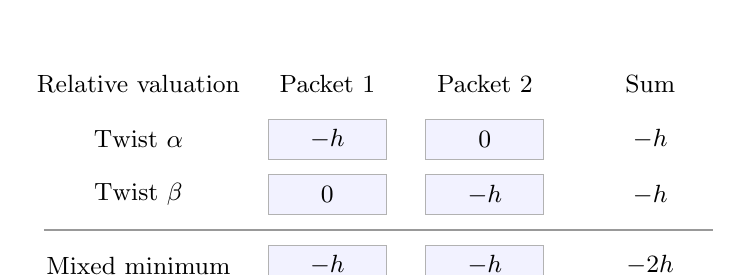
\begin{tikzpicture}[every node/.style={font=\small}]
\node at (0,1.3) {Relative valuation};\node at (2.4,1.3) {Packet 1};\node at (4.4,1.3) {Packet 2};\node at (6.5,1.3) {Sum};
\foreach \y/\label/\a/\b/\c in {0.6/Twist $\alpha$/$-h$/$0$/$-h$,-0.1/Twist $\beta$/$0$/$-h$/$-h$,-1.0/Mixed minimum/$-h$/$-h$/$-2h$}{\node at (0,\y){\label};\node[draw=black!30,fill=blue!5,minimum width=15mm,minimum height=5mm] at (2.4,\y){\a};\node[draw=black!30,fill=blue!5,minimum width=15mm,minimum height=5mm] at (4.4,\y){\b};\node at (6.5,\y){\c};}
\draw[black!40](-1.2,-0.55)--(7.3,-0.55);
\end{tikzpicture}
\end{center}
The formal polynomial is not itself a theta lift. Evaluation at integral values of $X$ can suffer cancellations (especially in small residue fields); the use of Gauss valuation avoids choosing a single evaluation at all. No automorphic object associated with the mixed variables is claimed.

\subsection{Global arithmetic ratio and determinant line}
Normalize the local absolute value by $|z|_\iota=p^{-v_\iota(z)}$ if $v_\iota(p)=1$. With $m_{\pi,\iota}=\min_\vartheta v_\iota(\lambda_{\pi,\vartheta})$, select a minimizing twist per packet and set
\begin{equation}\label{eq:ratio}
\mathcal R_\iota=\prod_\pi \lambda_{\pi,\vartheta(\pi,\iota)}^{-d_\pi}.
\end{equation}
Corollary \ref{cor:mixed} gives
\begin{equation}\label{eq:absratio}
|\det G_1|_\iota\leq p^{e_\iota}|\mathcal R_\iota|_\iota,
\qquad\log|\mathcal R_\iota|_\iota=(\log p)\sum_\pi d_\pi m_{\pi,\iota}.
\end{equation}
The sign is important: a smaller (more negative) valuation of the relative eigenvalue improves this upper bound on the finite-place absolute value of the reference determinant. If a pure-twist global height estimate holds for one common-cleared member at each prime, the mixed local minima are no worse with the same clearing. The prospective reduction is to produce a sufficient bound directly from packet-wise witnesses, without demanding one twist regular for every packet. Arbitrary local minimization does not by itself prove the global sum estimate. It is also necessary to use normalized local weights (local degrees divided by the coefficient field degree) in the product formula, and to check that all local ratios compare the same algebraic reference determinant. The ratios themselves may vary with $\iota$; the product formula is applied to the reference determinant, not to an invented common twist.

\subsection{The missing auxiliary basis and common clearing}
The actual short forms span only $h<D$ directions in a $D$-dimensional target. A basis completion $y_{h+1},\ldots,y_D$ needs arithmetic controls; the source permits twist-dependent correcting scalars $\gamma_\vartheta$ on these auxiliary forms. Mixed determinants require a common basis and common clearing. A sufficient local strategy is to choose one factor $\gamma$ with $v(\gamma)\geq\max_{\vartheta\in\mathcal T}v(\gamma_\vartheta)$, whenever each corresponding correcting scalar indeed suffices on the same auxiliary vectors. Then the extra clearing cost on that side is at most $(D-h)v(\gamma)$ if no other basis corrections are needed. For two sides charge both valuations. The small deficit $D-h\leq4D/b^2$ is useful only if the sum of these maximum local costs remains within the actual error budget. If the family requires new full-space clearing, the cost may outweigh the spectral gain; the intersection counterexample following \eqref{eq:clear} illustrates this. Finite families and common algebraic periods must be chosen explicitly. No summable bound for these common auxiliary corrections has been proved here.

\begin{obligation}[Packet-wise replacement of simultaneous selected twists]\label{obl:packets}
For the actual common target of the readable theta chain and each coefficient place, construct a finite admissible twist family and prove: (i) a common algebraic basis and normalization for relative operators; (ii) simultaneous triangularization with the exact Hecke multiplicities; (iii) common integral left and right corrections, including the short and complementary vectors; (iv) packet-wise valuations whose weighted local sums, together with the common clearing indices and reachable projection costs, obey the source's global selected-twist height bound. The actual $m$ successive powers of each twist, conductors, false-lift exclusion, exchange identities and all admissibility conditions must still hold for the relevant comparisons. Only then may this mechanism replace the source's simultaneous regular-family supplier.
\end{obligation}
The proof of \eqref{eq:gauss} is classical valuation algebra. Its application to this theta determinant route is the proposed structural refinement. We have not established publication priority or that the actual arithmetic witnesses become easier after this replacement. The open obligation is strictly weaker at the level of the abstract spectral minimum, but it could entail extra common-clearing or comparison requirements in practice.
\status{(P) Theorem \ref{thm:gauss}, Corollary \ref{cor:mixed}, signed ratio and examples; (S) the source Gram-chain and integral comparison interfaces as previously read; (C/O) Obligation \ref{obl:packets}.}
\section{The common determinant budget and the exact analytic endpoint}\label{sec:end}
\subsection{One signed comparison}
Let $y_1,\ldots,y_h$ be the selected independent short integral images in a target of dimension $D>0$, with $0<h\leq D$. Complete them by $D-h$ auxiliary vectors to a common basis. Let $C$ be an upper bound for the logarithm of their archimedean squared covolume, and $Q_{\rm comp}$ a corresponding complement cost. At each coefficient place the algebraic full-basis determinant is compared with the chosen twisted determinants after common left/right clearing. Write $I$ for the sum of the two clearing costs (in the symmetric case $I=2\delta$), and $B_{\rm ht}$ for the remaining global corrected ratio-height bound. The common determinant and product formula give
\begin{equation}\label{eq:budget}
0\leq C+I+Q_{\rm comp}+B_{\rm ht}.
\end{equation}
To see the bookkeeping, use a nonzero algebraic reference determinant $z$ in the full common basis. If its weighted archimedean log absolute values are bounded by $C+Q_{\rm comp}$ after the common algebraic normalization, and its weighted finite log absolute values by $I+B_{\rm ht}$, summing these two bounds and using $\sum_v w_v\log|z|_v=0$ proves \eqref{eq:budget}. The archimedean squared covolume of the short family is its Gram determinant; a basis completion has full Gram determinant equal to the short determinant times the determinant of the Gram matrix of the auxiliary vectors projected orthogonally off the short span (Schur complement). This justifies measuring the actual complement rather than its rank times its worst norm. Every period and algebraic scalar used to pass from this Gram determinant to $z$ must be retained on both sides. The mixed local bound \eqref{eq:absratio} is a candidate replacement for the finite-place part, with the common multiplier and normalized weights unchanged.

Suppose the analytic shortness and arithmetic comparison estimates are
\begin{equation}\label{eq:two}
C\leq h(H-mR+E_A),\qquad B_{\rm ht}\leq-DH+E_B,
\end{equation}
where $H$ is the common main term, $m>0$ the number of lifts, $R$ the signed prime remainder, and $E_A,E_B$ their actual error allowances. Then
\begin{equation}\boxed{hmR\leq-(D-h)H+hE_A+E_B+I+Q_{\rm comp}.}\label{eq:mainbudget}\end{equation}
This follows by substitution in \eqref{eq:budget}. If $H\geq0$, the missing-dimension term is favorable; without that sign it must not be discarded. Neither the absolute value of $R$ nor the lower sign is supplied by this inequality. This is the common comparison also described by Brox \cite{broxplan}; the source's \texttt{integral\_\allowbreak forms\_\allowbreak long} provides its lower-bound interface. More explicitly, the source sufficient estimates recorded in Brox's plan are
\begin{align*}
D(H-3L_0)&\leq C+2\delta, & C&\leq h(H-mR+L_0),\\
L_0&=fa(\log b)^4, & h&\geq(1-4/b^2)D,\\
\delta&\leq10D\log(1+2b^2)fa(\log b)^3, & H&\geq0.
\end{align*}
They imply $hmR\leq (3D+h)L_0+2\delta-(D-h)H$. For large $b$ in the prescribed parameter range this is bounded by $hfa(\log b)^5$, yielding $mR\leq fa(\log b)^5$. The complement cost is absorbed into that source interface; it should not be charged twice. The arithmetic hypotheses are not independently proved here. The proposed gain from reachable defects and mixed twists is an improvement or replacement of the lower comparison supplier, not a change to the elementary signed cancellation.

\subsection{The signed prime remainder: normalization and transform}
The analytic endpoint below is reconstructed from the readable source interface and Brox's zero-detection note \cite{broxzero}. Fix a modulus $q_0$ and a nonprincipal primitive quadratic Dirichlet character $\chi$ of conductor coprime to $q_0$. Put $\varphi=\varphi(q_0)$ and let $\psi$ range over all characters modulo $q_0$, including imprimitive ones. Define
\[
E_\psi(s)=\begin{cases}(s-1)L(s,\psi)&\psi\text{ principal},\\L(s,\psi)&\text{otherwise},\end{cases}\quad
P(s)=\prod_{\psi\bmod q_0}E_\psi(s),\quad Q_\chi(s)=\prod_{\psi\bmod q_0}E_{\psi\chi}(s).
\]
At $s=1$ the principal factor is interpreted by analytic continuation. Classical Dirichlet $L$-function theory supplies entire factors with nonzero value at $1$ and no zeros for $\Re s\geq1$. The products $\psi\chi$ are nonprincipal by the coprime-conductor condition. Set
\begin{align}
a_\chi(n)&=\Lambda(n)(1-\chi(n))\mathbf1_{n\equiv1\ (q_0)},\\
G_\chi(s)&=\frac{1}{\varphi}\left(\frac{Q_\chi'}{Q_\chi}(s)-\frac{P'}P(s)-1\right),\qquad c_\chi=G_\chi(1),\\
R_\chi(x)&=\sum_{n\leq x}a_\chi(n)\left(\frac1n-\frac1x\right)-\frac{\log x}{\varphi}-c_\chi.\label{eq:prime}
\end{align}
Complex-conjugation invariance makes the constant real. Its subtraction is essential; replacing it by an arbitrary additive constant destroys the required decaying remainder. The arithmetic argument must target this exact normalization rather than an unrelated signed prime sum.

\begin{proposition}[Mellin transform and residue]\label{prop:mellin}
For $\Re s>1$,
\begin{equation}\label{eq:mellin}
\Phi_\chi(s):=\int_1^\infty R_\chi(x)x^{-s}\,dx=\frac{G_\chi(s)/s-c_\chi}{s-1}.
\end{equation}
The right-hand side is meromorphic in $\Re s>0$, has at most simple poles and is regular at $s=1$. At $\rho\ne1$ its residue is
\begin{equation}\label{eq:resid}
r_\chi(\rho)=\frac{\operatorname{ord}_\rho P-\operatorname{ord}_\rho Q_\chi}{\varphi\rho(1-\rho)}.
\end{equation}
\end{proposition}
\begin{proof}
By character orthogonality and absolute convergence, $F_\chi(s)=\sum_{n\geq1}a_\chi(n)n^{-s}=G_\chi(s)+s/[\varphi(s-1)]$. The termwise integral of $(1/n-1/x)\mathbf1_{x\geq n}x^{-s}$ is $n^{-s}/[s(s-1)]$. The logarithmic term integrates to $1/[\varphi(s-1)^2]$, and the constant term to $c_\chi/(s-1)$. Substitution proves \eqref{eq:mellin}. Since its numerator vanishes at $1$, the apparent singularity there is removable. A logarithmic derivative of a holomorphic function has simple poles with residues equal to the zero multiplicities. Applying that fact to $G_\chi$ proves \eqref{eq:resid} with the displayed sign.
\end{proof}

\begin{lemma}[One-sided Landau argument]\label{lem:landau}
Suppose a real measurable $E(t)$ on $t\geq0$ satisfies $|E(t)|\leq C_0e^t$ and $E(t)\leq C_1e^{(\beta-1)t}$ eventually. Assume its transform $\Phi(s)=\int_0^\infty E(t)e^{(1-s)t}\,dt$ has a meromorphic continuation to $\Re s>0$ with only simple poles and nonnegative real residue at each real $s>\beta>0$. Then $\Phi$ is holomorphic for $\Re s>\beta$.
\end{lemma}
\begin{proof}
Choose $K_0$ large enough that $K_0e^{\beta t}-e^tE(t)\geq0$ everywhere, using the growth bound on the finite initial interval. Its positive Laplace transform $\Psi(s)=K_0/(s-\beta)-\Phi(s)$ initially agrees far to the right. Let $a$ be the real abscissa of convergence. If $a>\beta$, the possible simple pole at $a$ has nonpositive residue from the assumed residue sign for $\Phi$. Positivity on the real axis to its right forces that residue to be nonnegative, hence zero. Thus $\Psi$ is analytic at $a$. But a positive Laplace transform cannot be analytic there: if analytic in a disc around $a$, take real $z>a$ sufficiently close to $a$ so the Taylor series about $z$ converges at some real $\sigma<a$. The derivative integrals, with alternating signs, are its moments at $z$. Expanding $e^{(z-\sigma)t}$ into its nonnegative series and applying monotone convergence yields convergence of the Laplace integral at $\sigma$, a contradiction. Thus $a\leq\beta$ (or $a=-\infty$) and the positive Laplace transform, hence $\Phi$, is holomorphic in the asserted half-plane.
\end{proof}
The sign condition is necessary: $E(t)=e^{(a-1)t}(\cos(\tau t)-1)\leq0$ for $\beta<a<1$, $\tau\ne0$, has transform $(s-a)/((s-a)^2+\tau^2)-1/(s-a)$, with a negative real residue at $a$ and nonreal poles in the prohibited half-plane. A one-sided bound by itself is insufficient.

Apply the lemma to $E(t)=R_\chi(e^t)$ with $1/2<\beta<1$. Growth follows from the elementary bound
\[\sum_{n\leq x}\Lambda(n)/n=O(1+(\log x)^2).\] If $R_\chi(x)\leq Cx^{\beta-1}$ eventually and the real multiplicities satisfy $\operatorname{ord}_t Q_\chi\leq\operatorname{ord}_t P$ for $\beta<t<1$, the residues in \eqref{eq:resid} satisfy the sign hypothesis. Therefore the two products have equal zero multiplicities everywhere in $\Re s>\beta$. To exclude a proposed zero $\rho$ of $P$ it is enough to select a fixed $\chi$ such that $Q_\chi$ has no zeros in $\Re s\geq\beta$, $|\Im s|\leq|\Im\rho|$; the real multiplicity condition and unequal multiplicity at $\rho$ are the actual weaker requirements. All character factors must be included; otherwise cancellation between factors is unaccounted for.

Brox proves the finite-box selection from classical ingredients \cite{broxzero}: for $8\mid q_0$, any allowed prime progression $d\equiv a_0\pmod{q_0}$ with $a_0\equiv7\pmod8$, and fixed $\beta,H_0$, infinitely many such primes have all $L(s,\psi\chi_d)$ nonzero on the stated bounded-height half-strip, with $\chi_d(n)=(n/d)$. The proof uses theta transforms, a truncated M\"obius theta integral, three-lines, a Jacobi-symbol second moment and prime counts in fixed progressions. This is an external supplier here, not a new nonvanishing claim. It lets us fix the quadratic character before the main scale $x$ grows. In the actual readable-source setting the admissible modulus is divisible by $18480$ and the auxiliary prime is in its specified class (the ordinary RH test can start with $q_0=18480$, not $q_0=1$). This fixed modulus contains the principal factor and hence the nontrivial zeros of zeta; finite Euler factors of imprimitive characters introduce no zeros in the open strip.

\subsection{From the arithmetic remainder to RH}
The source's exact prime identity, as recorded in \cite{broxplan}, has the sufficient bound
\begin{equation}\label{eq:finalprime}
R_{q_0,d}(x)\leq \frac{\varphi(q_0)(\log b)^6}{m}+|R_{q_0,d}(x_1)|+\log b\,|R_{1,d}(x_1)|.
\end{equation}
The actual data must exist for all sufficiently large integers $x$ at each fixed accuracy, with $m\geq\sqrt{x}$, $\log b\ll x^\varepsilon$ and $\log x_1\geq x^{\varepsilon/12}$. The last two terms are superpolynomially small in $x$ by the classical fixed-modulus prime number theorem in its usual effective decay form for the fixed $q_0,d$ (constants may depend on them). Thus the bound has exponent $-1/2+6\varepsilon$ for the normalized $R$ in \eqref{eq:prime}. Interpolation from integers is harmless here: for $n<x<n+1$, the finite sum has derivative $x^{-2}\sum_{j\leq n}a_\chi(j)$, so by the usual Chebyshev estimate it and the logarithmic derivative are $O(1/x)$. One may choose $\varepsilon$ small compared with $\Re\rho-1/2$ to apply Lemma \ref{lem:landau}. Functional-equation symmetry then yields RH. This is a conditional completion, not a claim that the data needed for \eqref{eq:finalprime} have been constructed by this manuscript. The unnormalized prime error and the normalized $R$ must not be confused: the desired one-sided remainder here decays as $x^{-1/2+o(1)}$, not grows as $x^{1/2+o(1)}$.
\status{(P) the determinant-budget algebra and the elementary analytic derivations under their hypotheses; (S) the exact source remainder interface and finite-box selection; (O) the uniform arithmetic construction needed to establish \eqref{eq:finalprime} independently.}

\section{Dependency ledger and prioritized reconstruction tasks}\label{sec:ledger}
The following is a mathematical acceptance ledger, not a percentage of proof completion. The local kernel bound, global class-sum comparison and arithmetic integrality are not interchangeable. Each replacement must use the same source and target, level, coefficient fields, scales and Haar measures. The formal source provides theorems but a human-auditable reconstruction still needs ordinary proofs or explicitly stated standard theorems with verified hypotheses.
\begin{longtable}{p{0.24\textwidth}p{0.14\textwidth}p{0.52\textwidth}}
\toprule\textbf{Object}&\textbf{Status}&\textbf{Acceptance requirement / result}\\\midrule\endhead
Exact geometric scales & P/S & Norm of the different, exact prefix products, Poisson normalization, \eqref{eq:kappa}--\eqref{eq:poissprod}.\\
Ideal packing and Bessel summation & P/C & Theorems \ref{thm:packing}, \ref{thm:bessel}; local kernel hypotheses retained. No separate S-unit classification necessary.\\
Weighted convolution and head control & P/C & Reciprocal grouping, norm prefix bounds, exact depth recurrence, first-coordinate dominance.\\
F1: local coupled kernel & O & Derive the archimedean Bessel transform bound and finite orbital-density realization in the exact source conventions; prove joint positivity and support where needed.\\
F2: global moments & O & Siegel comparison, remaining Bruhat cells, near returns, correct target multiplicities and translate probability measure. Match every factor with the actual Poincar\'e map.\\
Ramified persistent spanning & P/C & Retain compression and saturated selection, prove actual first-moment loss and translate-wise deficit/second moment. Match the source's $(1-4/b^2)D$ rank and shortness budget.\\
F3: integral theta diagram & O & Common-scalar seesaw, integral jet divisibilities and simultaneous lattice index estimates. Prove actual selected-image clearing cost.\\
Reachable torsion & P/C & Exact signed local formula \eqref{eq:signed}; establish the actual period-lattice image bound or containment \eqref{eq:vanish}.\\
Finite Selmer presentation & P/C & Common finite quotient, polynomial linear equations and sharp maximal minor; check normalization and local arithmetic conditions.\\
F4: bounded witnesses & O & Actual tied module and $\beta_T$, integral matrix span, local crystalline rank budget, coefficient uniformity and projection denominator. Degree-independent selection is an external available supplier.\\
Mixed determinants & P/C & Common Gauss formula and strict-gain example. Verify actual relative Hecke operators and shared algebraic pairing.\\
F5: determinant transport & O & False-lift exclusion, one-lift gluing and exchanges, chain Hecke-value ratios; common auxiliary corrections and summable mixed height per Obligation \ref{obl:packets}.\\
Final signed budget and analytic detection & P/S/C & Retain the exact common multiplier, missing-dimension sign and normalized prime sum. Establish arithmetic data for all sufficiently large $x$ after fixing accuracy and auxiliary character.\\\bottomrule
\end{longtable}
These five substantive suppliers are not asserted to be mathematically irreducible. The point of the ledger is to expose what remains to be eliminated. In the preferred route, the original W10 geometric wall/divisor machinery is no longer mandatory; the determinant route still needs a legitimate arithmetic lower bound. The original uniform untwisted Selmer and geometric height research can be imported only after checking the exact field/lattice/map dictionary. Brox's public frontier explicitly separates those alternative branches and warns that local constructions do not close the complete RH node \cite{broxfrontier}.

The next experiments should be carried out on the actual source objects in this order. First, identify the finite orbital-density features and archimedean Bessel features on common heads; use the proven packing-convolution bound to avoid reconstructing redundant global frequency-counting lemmas. Second, derive the centered trace or the precise source deficit and second moment, paying particular attention to non-main and near-return classes. Third, derive the reachable map $gJ$ on the integral period lattice and test whether its image intersects the complementary good-lift lattice sufficiently deeply for signed index cancellation. Fourth, use the actual Hecke-chain operators to prove or refute simultaneous relative triangularization in the common coefficient basis, then try packet-wise witnesses and charge their common auxiliary clearing. An arbitrarily attractive mixed-twist valuation profile is of no use if the common basis costs consume the gain. These tests address concrete suppliers rather than introduce another equivalent formulation of RH.

\section{Conceptual synthesis and novelty audit}\label{sec:novelty}
The initial physical and engineering analogies are useful because they lead to precise, falsifiable statements. The cascade-filter picture led to depth-resolved decay \eqref{eq:depth}; the product formula gives arithmetic exclusion of simultaneous small frequencies. Interference led to the character identity \eqref{eq:char}, whose genuine arithmetic symmetry must be verified. Complementary sensing led to tensor Gram coherence and persistent selection. The differential-amplifier picture led to the centered energy \eqref{eq:center} and early cancellation of the main term in \eqref{eq:mainbudget}. Electrical-network elimination failed without relative coercivity, as the explicit Schur-complement counterexample shows. Statistical mechanics suggests the competition of logarithmic complexity $400n^9 f\log b$ against the depth suppression $19Kf\log b$; here $k\asymp x^5$ versus $n^9=O(x^{4.5})$ supplies an actual asymptotic separation. The physics of a hypothetical zero $\rho=1/2+\delta+i\gamma$ suggests a square-root-normalized mode growing like $x^\delta$ in logarithmic time, but a single-mode picture cannot rule out cancellation between zeros; the exact Landau argument supplies the appropriate analytic endpoint. None of these analogies is a substitute for arithmetic hypotheses.

Volume is a plausible common organizing quantity, but different volumes must be distinguished. The ideal-packing quantity $V$ is a scaled norm product, the archimedean Gram determinant is a squared covolume, and the local arithmetic lattice determinant measures signed valuations. The product formula applies to a nonzero algebraic determinant after the correct common normalization, not to an arbitrary positive real volume. Proposition \ref{prop:glue} explains the exact compression balance and Theorem \ref{thm:signed} isolates the reachable arithmetic cost. The mixed determinant formula \eqref{eq:gauss} shows that complementary realizations can jointly strengthen a finite-place bound without integral spectral projectors. The Hensel counterexample proves that volume conservation alone does not force the arithmetic defects to be small.

Precedents in geometry of numbers include Skriganov's admissible-lattice theory, the counts of Barroero and Widmer, and Widmer's number-field ideal lattice estimates \cite{skriganov,barroero,widmerweak,widmercount}. Arakelov degree and determinant-line arithmetic are established subjects, as are Gauss valuations, Smith normal form, the Schur product theorem and the product formula. The present work makes no priority claim for those ingredients. The potentially distinctive contributions are their specific combination into the field-uniform coupled Bessel estimate, exact head-prefix and depth budget, reachable congruence image, and mixed-twist optimization proposed for this particular theta proof architecture. No exhaustive novelty search or referee review has been completed. The source itself already performs operator-valued clearing and a determinant comparison, so replacing a scalar denominator by a colength alone is not a new contribution. The more precise candidate improvement is restricting the colength to the reached submodule and moving twist optimization inside the packet sum while keeping the common clearing budget.

\section{Conclusion}
The strongest independently proved results of this manuscript are the norm-based ideal-packing theorem, its integrated coupled-frequency bound conditional on the actual local majorant, the exact head and convolution inequalities, the persistent selection lemmas, the signed local index formula and the mixed determinant Gauss identity. Their role is to reduce the complexity of the ordinary reconstruction rather than to claim that the theorem follows solely from elementary facts. The final conditional determinant comparison and analytic endpoint are explicit. The remaining substantive work is F1--F5 of Section \ref{sec:ledger}, in particular the local/global Bessel realization, simultaneous integral seesaw, tied arithmetic witnesses and the mixed-height compatibility of the actual theta maps. A complete independent proof of RH has not been obtained in this manuscript.

\paragraph{Reproducibility and authoring note.} This manuscript consolidates the author's recent research programme and AI-assisted mathematical working notes. The pinned readable source's scale, frequency, head-weight and recurrence declarations and the downstream Siegel normalization were inspected during preparation. The remaining theta/Selmer declaration names are retained from prior source readings as navigation anchors, and their full arithmetic proofs have not been independently replayed or translated here. The manuscript includes all derived mathematical interfaces and their limitations; it does not certify novelty or independent kernel verification. The source tree, third-party verification reports and dated Brox notes below permit the next audit. No reliance on RH as an input is intended for any independent lemma.

\appendix
\section{Source navigation and exact interfaces}\label{app:source}
The following crosswalk is intended to make the manuscript independently auditable. For the first two files use the readable tree \texttt{grh/\allowbreak src/\allowbreak New} at the pinned revision; line numbers can differ between GitHub display and raw file. The remaining file/symbol pairs are retained source navigation anchors from the preceding research notes; their full signatures and namespaces must be checked before a formal replacement. They are not newly proved theorems of this manuscript.
\begin{longtable}{p{0.35\textwidth}p{0.57\textwidth}}
\toprule\textbf{Source location}&\textbf{Interface to retain}\\\midrule\endhead
\texttt{Spanning/\allowbreak MainTerm/\allowbreak  GlobalSieve.lean}&\texttt{frequencyDecay}, \texttt{frequency\_\allowbreak term\_\allowbreak le}, \texttt{sum\_\allowbreak frequencies\_\allowbreak le}, \texttt{prod\_\allowbreak abs\_\allowbreak realM}, \texttt{boundsDecay\_\allowbreak prod}: exact finite and infinite factors; scale and admissibility.\\
Same file&\texttt{poissonConst}, \texttt{entryDensity}, \texttt{densitySum}, \texttt{densitySum\_\allowbreak succ\_\allowbreak le}, \texttt{re\_\allowbreak le\_\allowbreak of\_\allowbreak last\_\allowbreak entries\_\allowbreak ne}, \texttt{re\_\allowbreak sum\_\allowbreak sum\_\allowbreak le\_\allowbreak densitySum\_\allowbreak add}: common-entry Poisson and off-diagonal recurrence.\\
Same file&\texttt{headProduct}, \texttt{globalWeight}, \texttt{headProduct\_\allowbreak injective}, \texttt{isIntegral\_\allowbreak headProduct\_\allowbreak and\_\allowbreak norm\_\allowbreak le}, \texttt{sq\_\allowbreak sum\_\allowbreak globalWeight\_\allowbreak le}: actual support and head costs.\\
\texttt{Spanning/\allowbreak MainTerm/\allowbreak  EnergyEstimate.lean}&\texttt{prod\_\allowbreak poissonConst\_\allowbreak eq}, \texttt{scaledSiegelConst\_\allowbreak mul\_\allowbreak decayConst\_\allowbreak le}, \texttt{mul\_\allowbreak sum\_\allowbreak norm\_\allowbreak sum\_\allowbreak cosetAmplitude\_\allowbreak sq\_\allowbreak le}: precise downstream normalization and Siegel comparison.\\
\texttt{ShortAndEnough.lean}&Original selection, translate count, retained dimensions, ramified codimension.\\
\texttt{SeesawIdentity.lean}&\texttt{New.Data.seesaw\_\allowbreak identity}: exact common scalar and finite chain data.\\
Integral composite lift declarations&\texttt{New.Data.exists\_\allowbreak err\_\allowbreak gaugeLe\_\allowbreak compositeLift}: simultaneous local gauge and total loss.\\
\texttt{IntegralTargetForms.lean}, \texttt{TwistedLattice.lean}&Simultaneous pullback integrality, false-lift and congruence comparison.\\
\texttt{LongForms.lean}, \texttt{LiftVolumeHeight.lean}&\texttt{New.Data.integral\_\allowbreak forms\_\allowbreak long}; common-basis determinant, auxiliary vectors, local selected twist, integral projection defects.\\
\texttt{NormOfChain.lean}&Hecke operators, relative norms and chain multiplicities.\\
\texttt{Congruences/\allowbreak Selmer/\allowbreak  OneSystem.lean}, \texttt{Line.lean}, \texttt{GeneralTheorem.lean}&\texttt{exists\_\allowbreak matrix\_\allowbreak selmerAtPoint\_\allowbreak equiv}, \texttt{exists\_\allowbreak sharp\_\allowbreak polynomial}, tied-module witness, actual \texttt{SelmerDatum} and \texttt{TwistedLengthLe} assumptions.\\\bottomrule
\end{longtable}

\begin{thebibliography}{99}
\bibitem{sernau} L. Sernau et al. (with Anthropic and Claude), \emph{A short Lean 4 proof of the Generalized Riemann Hypothesis}, 25 November 2026. Readable and compact editions, revision \texttt{72fead102f663d5c7a407964a13dc0cf9d977207}. \url{https://github.com/lsernau/grh-lean}.
\bibitem{sutherland} A. V. Sutherland, \emph{Verification files for the shorter Lean proof of RH and of GRH for Dirichlet L-functions}, MIT, report updated 26 November 2026. \url{https://math.mit.edu/~drew/shortgrh/}.
\bibitem{rubinstein} M. Rubinstein, \emph{Alp\"oge/Claude proof of the Generalized Riemann Hypothesis}, public reading and verification resources, November 2026. \url{https://www.math.uwaterloo.ca/~mrubinst/alpoge_claude_grh/}.
\bibitem{globalsieve} Sernau et al., readable Lean source, \emph{GlobalSieve.lean}, pinned revision as in [1]. \url{https://github.com/lsernau/grh-lean/blob/72fead102f663d5c7a407964a13dc0cf9d977207/grh/src/New/Spanning/MainTerm/GlobalSieve.lean}.
\bibitem{energy} Sernau et al., readable Lean source, \emph{EnergyEstimate.lean}, pinned revision as in [1]. \url{https://github.com/lsernau/grh-lean/blob/72fead102f663d5c7a407964a13dc0cf9d977207/grh/src/New/Spanning/MainTerm/EnergyEstimate.lean}.
\bibitem{broxplan} J. Brox, \emph{Preferred proof plan: short forms, spanning, and one determinant}, revised 26 November 2026, GRH\_distillation. \url{https://github.com/JoseBrox/GRH_distillation/blob/main/blueprint/merged-proof-plan.md} (accessed 27 November 2026).
\bibitem{broxfrontier} J. Brox, \emph{Open frontier theorems}, GRH\_distillation. \url{https://github.com/JoseBrox/GRH_distillation/blob/main/notes/open-frontier-theorems.md} (accessed 27 November 2026).
\bibitem{broxzero} J. Brox, \emph{Zero detection for the readable Sernau route}, GRH\_distillation, note \texttt{lsernau-zero-detection.md}. \url{https://github.com/JoseBrox/GRH_distillation/blob/main/notes/lsernau-zero-detection.md} (accessed 27 November 2026).
\bibitem{broxtorsion} J. Brox, \emph{Degree-independent torsion specialization}, GRH\_distillation, note \texttt{lsernau-twist-specialization.md}. \url{https://github.com/JoseBrox/GRH_distillation/blob/main/notes/lsernau-twist-specialization.md} (accessed 27 November 2026).
\bibitem{skriganov} M. M. Skriganov, \emph{Constructions of uniform distributions in terms of geometry of numbers}, Algebra i Analiz 6 (1994), English translation in St. Petersburg Math. J. 6 (1995).
\bibitem{barroero} F. Barroero and M. Widmer, \emph{Counting lattice points and o-minimal structures}, Int. Math. Res. Not. (2014).
\bibitem{widmerweak} M. Widmer, \emph{Weak admissibility, primitivity, o-minimality, and Diophantine approximation}, Mathematika 64 (2018), doi:\href{https://doi.org/10.1112/S0025579318000049}{10.1112/S0025579318000049}.
\bibitem{widmercount} M. Widmer, \emph{Counting bounded elements of a number field}, Int. Math. Res. Not. 2022(1), 373 ff. \url{https://academic.oup.com/imrn/article-abstract/2022/1/373/5859244}.
\bibitem{beukers} F. Beukers and H. P. Schlickewei, \emph{The equation $x+y=1$ in finitely generated groups}, Acta Arith. 78 (1996), 189--199.
\end{thebibliography}
\end{document}
